% Journal manuscript draft (IEEEtran journal). Every result below is a macro
% (generated/numbers.tex) or a table fragment (generated/tbl_*.tex) produced from
% the frozen result files by scripts/build_paper_numbers.py and
% scripts/build_paper_tables.py. Do not type a result into the text. Typed numbers
% are cohort facts, configuration constants or pre-registered thresholds.
% References: IEEE style, numbered in order of first citation. After editing, run
%   python scripts/order_bibitems.py paper/main_journal.tex
% to restore first-citation order. Entries were checked against publisher or
% index pages on 2026-11-19; items still to confirm are marked with a comment.
\documentclass[journal]{IEEEtran}
\IEEEoverridecommandlockouts
\usepackage{cite}
% Times text as in IEEEtran under pdfLaTeX; under XeTeX (tectonic) load the same face.
\usepackage{iftex}
\ifPDFTeX\else\usepackage{fontspec}\setmainfont{texgyretermes}[Extension=.otf,UprightFont=*-regular,BoldFont=*-bold,ItalicFont=*-italic,BoldItalicFont=*-bolditalic]\fi
\usepackage{amsmath,amssymb,amsfonts}
\usepackage{algorithmic}
\usepackage{graphicx}
\usepackage{textcomp}
\usepackage{xcolor}
\usepackage{booktabs}
\usepackage{array}
\usepackage{microtype}
\usepackage{enumitem}
\usepackage{tikz}
\usetikzlibrary{positioning,arrows.meta}
\usepackage[hidelinks]{hyperref}
% Generated by scripts/build_paper_numbers.py. Do not edit by hand.
\newcommand{\numBootDraws}{2000}
\newcommand{\numCOneDeltaZeroEight}{-0.124}
\newcommand{\numCOneDeltaZeroFive}{-0.048}
\newcommand{\numCOneDeltaZeroNine}{-0.169}
\newcommand{\numCOneDeltaZeroSeven}{-0.103}
\newcommand{\numCOneDeltaZeroSix}{-0.058}
\newcommand{\numCThreeDeltaZeroEight}{-0.088}
\newcommand{\numCThreeDeltaZeroFive}{-0.027}
\newcommand{\numCThreeDeltaZeroNine}{-0.124}
\newcommand{\numCThreeDeltaZeroSeven}{-0.069}
\newcommand{\numCThreeDeltaZeroSix}{-0.042}
\newcommand{\numCThreeUpperZeroEight}{-0.043}
\newcommand{\numCThreeUpperZeroFive}{-0.006}
\newcommand{\numCThreeUpperZeroNine}{-0.066}
\newcommand{\numCThreeUpperZeroSeven}{-0.036}
\newcommand{\numCThreeUpperZeroSix}{-0.015}
\newcommand{\numDiceCoreREight}{0.605}
\newcommand{\numDiceCoreRSeven}{0.409}
\newcommand{\numDiceCoreRTwo}{0.390}
\newcommand{\numDiceEnhREight}{0.799}
\newcommand{\numDiceEnhRSeven}{0.481}
\newcommand{\numDiceEnhRTwo}{0.431}
\newcommand{\numDiceOedREight}{0.819}
\newcommand{\numDiceOedRSeven}{0.566}
\newcommand{\numDiceOedRTwo}{0.597}
\newcommand{\numDiceREight}{0.741}
\newcommand{\numDiceRSeven}{0.485}
\newcommand{\numDiceRTwo}{0.473}
\newcommand{\numExtAbstAlphafive}{0.525}
\newcommand{\numExtAbstAlphaten}{0.243}
\newcommand{\numExtAbstAlphatwenty}{0.163}
\newcommand{\numExtAlwaysCeFlair}{0.208}
\newcommand{\numExtAlwaysDropFlair}{0.203}
\newcommand{\numExtAlwaysDropTone}{0.163}
\newcommand{\numExtAlwaysDropTonece}{0.450}
\newcommand{\numExtAlwaysDropTtwo}{0.129}
\newcommand{\numExtAlwaysFull}{0.153}
\newcommand{\numExtAurcCeFlair}{0.064}
\newcommand{\numExtAurcDropFlair}{0.101}
\newcommand{\numExtAurcDropTone}{0.058}
\newcommand{\numExtAurcDropTonece}{0.310}
\newcommand{\numExtAurcDropTtwo}{0.040}
\newcommand{\numExtAurcFull}{0.051}
\newcommand{\numExtAurcHi}{0.081}
\newcommand{\numExtAurcLo}{0.029}
\newcommand{\numExtAurcMFiveCeFlair}{0.064}
\newcommand{\numExtAurcMFiveDropFlair}{0.101}
\newcommand{\numExtAurcMFiveDropTone}{0.058}
\newcommand{\numExtAurcMFiveDropTonece}{0.310}
\newcommand{\numExtAurcMFiveDropTtwo}{0.040}
\newcommand{\numExtAurcMFiveFull}{0.051}
\newcommand{\numExtAurcMFourCeFlair}{0.270}
\newcommand{\numExtAurcMFourDropFlair}{0.175}
\newcommand{\numExtAurcMFourDropTone}{0.112}
\newcommand{\numExtAurcMFourDropTonece}{0.393}
\newcommand{\numExtAurcMFourDropTtwo}{0.173}
\newcommand{\numExtAurcMFourFull}{0.120}
\newcommand{\numExtAurcMOneCeFlair}{0.064}
\newcommand{\numExtAurcMOneDropFlair}{0.101}
\newcommand{\numExtAurcMOneDropTone}{0.058}
\newcommand{\numExtAurcMOneDropTonece}{0.310}
\newcommand{\numExtAurcMOneDropTtwo}{0.040}
\newcommand{\numExtAurcMOneFull}{0.051}
\newcommand{\numExtAurcMSixCeFlair}{0.083}
\newcommand{\numExtAurcMSixDropFlair}{0.255}
\newcommand{\numExtAurcMSixDropTone}{0.065}
\newcommand{\numExtAurcMSixDropTonece}{0.589}
\newcommand{\numExtAurcMSixDropTtwo}{0.078}
\newcommand{\numExtAurcMSixFull}{0.092}
\newcommand{\numExtAurcMThreeCeFlair}{0.065}
\newcommand{\numExtAurcMThreeDropFlair}{0.105}
\newcommand{\numExtAurcMThreeDropTone}{0.061}
\newcommand{\numExtAurcMThreeDropTonece}{0.290}
\newcommand{\numExtAurcMThreeDropTtwo}{0.039}
\newcommand{\numExtAurcMThreeFull}{0.051}
\newcommand{\numExtAurcMTwoCeFlair}{0.064}
\newcommand{\numExtAurcMTwoDropFlair}{0.101}
\newcommand{\numExtAurcMTwoDropTone}{0.058}
\newcommand{\numExtAurcMTwoDropTonece}{0.310}
\newcommand{\numExtAurcMTwoDropTtwo}{0.040}
\newcommand{\numExtAurcMTwoFull}{0.051}
\newcommand{\numExtAurocHi}{0.970}
\newcommand{\numExtAurocLo}{0.888}
\newcommand{\numExtBrierMOne}{0.118}
\newcommand{\numExtBrierMTwo}{0.121}
\newcommand{\numExtCOneDiff}{-0.025}
\newcommand{\numExtCOneHi}{0.021}
\newcommand{\numExtCOneLo}{-0.078}
\newcommand{\numExtCalCovAlphafive}{0.960}
\newcommand{\numExtCalCovAlphaten}{0.911}
\newcommand{\numExtCalCovAlphatwenty}{0.806}
\newcommand{\numExtCovAlphafive}{0.985}
\newcommand{\numExtCovAlphaten}{0.931}
\newcommand{\numExtCovAlphatwenty}{0.738}
\newcommand{\numExtDTwoAbs}{0.0034}
\newcommand{\numExtDTwoDiff}{-0.0034}
\newcommand{\numExtEFourDiff}{0.025}
\newcommand{\numExtEOneDiff}{-0.024}
\newcommand{\numExtEThreeDiff}{-0.002}
\newcommand{\numExtETwoDiff}{0.040}
\newcommand{\numExtEceMOne}{0.097}
\newcommand{\numExtEceMOneHi}{0.146}
\newcommand{\numExtEceMOneLo}{0.076}
\newcommand{\numExtEceMTwo}{0.106}
\newcommand{\numExtEceMTwoHi}{0.160}
\newcommand{\numExtEceMTwoLo}{0.091}
\newcommand{\numExtEmptyAlphafive}{0}
\newcommand{\numExtEmptyAlphaten}{0}
\newcommand{\numExtEmptyAlphatwenty}{33}
\newcommand{\numExtFullAlphafive}{106}
\newcommand{\numExtFullAlphaten}{49}
\newcommand{\numExtFullAlphatwenty}{0}
\newcommand{\numExtHalfAlphafive}{0.042}
\newcommand{\numExtHalfAlphafiveCeFlair}{0.020}
\newcommand{\numExtHalfAlphafiveDropFlair}{0.064}
\newcommand{\numExtHalfAlphafiveDropTone}{0.042}
\newcommand{\numExtHalfAlphafiveDropTonece}{0.136}
\newcommand{\numExtHalfAlphafiveDropTtwo}{0.015}
\newcommand{\numExtHalfAlphafiveFull}{0.042}
\newcommand{\numExtHalfAlphaten}{0.079}
\newcommand{\numExtHalfAlphatwenty}{0.141}
\newcommand{\numExtOracle}{0.013}
\newcommand{\numExtQuantAlphafive}{0.777}
\newcommand{\numExtQuantAlphaten}{0.662}
\newcommand{\numExtQuantAlphatwenty}{0.392}
\newcommand{\numExtREightAurc}{0.076}
\newcommand{\numExtREightAuroc}{0.927}
\newcommand{\numExtREightBrier}{0.135}
\newcommand{\numExtREightEce}{0.135}
\newcommand{\numExtRSevenAurc}{0.090}
\newcommand{\numExtRSevenAuroc}{0.904}
\newcommand{\numExtRSevenBrier}{0.137}
\newcommand{\numExtRSevenEce}{0.117}
\newcommand{\numExtRTwoAurc}{0.051}
\newcommand{\numExtRTwoAuroc}{0.929}
\newcommand{\numExtRTwoBrier}{0.121}
\newcommand{\numExtRTwoEce}{0.106}
\newcommand{\numExtRefitCovAlphafive}{0.985}
\newcommand{\numExtRefitCovAlphaten}{0.931}
\newcommand{\numExtRefitCovAlphatwenty}{0.738}
\newcommand{\numExtRiskZeroEight}{0.111}
\newcommand{\numExtRiskZeroFive}{0.030}
\newcommand{\numExtRiskZeroNine}{0.126}
\newcommand{\numExtRiskZeroSeven}{0.085}
\newcommand{\numExtRiskZeroSix}{0.066}
\newcommand{\numExtSingleTrueAlphafive}{0.969}
\newcommand{\numExtSingleTrueAlphaten}{0.908}
\newcommand{\numExtSingleTrueAlphatwenty}{0.882}
\newcommand{\numFamUAOneAdj}{0.243}
\newcommand{\numFamUAThreeAdj}{0.964}
\newcommand{\numFamUATwoAdj}{0.958}
\newcommand{\numFamUBFiveAdj}{0.263}
\newcommand{\numFamUBFourAdj}{0.267}
\newcommand{\numFamUBOneAdj}{0.985}
\newcommand{\numFamUBThreeAdj}{0.941}
\newcommand{\numFamUBTwoAdj}{0.005}
\newcommand{\numFamUDOneAdj}{0.842}
\newcommand{\numFamUDTwoAdj}{0.580}
\newcommand{\numFamUEFourAdj}{0.258}
\newcommand{\numFamUEOneAdj}{0.811}
\newcommand{\numFamUEThreeAdj}{0.811}
\newcommand{\numFamUETwoAdj}{0.748}
\newcommand{\numFamXAOneAdj}{0.960}
\newcommand{\numFamXAThreeAdj}{0.005}
\newcommand{\numFamXATwoAdj}{0.005}
\newcommand{\numFamXBFiveAdj}{0.457}
\newcommand{\numFamXBFourAdj}{0.012}
\newcommand{\numFamXBOneAdj}{0.258}
\newcommand{\numFamXBThreeAdj}{0.411}
\newcommand{\numFamXBTwoAdj}{0.005}
\newcommand{\numFamXCOneAdj}{0.457}
\newcommand{\numFamXDOneAdj}{0.411}
\newcommand{\numFamXDTwoAdj}{0.005}
\newcommand{\numFamXEFourAdj}{0.152}
\newcommand{\numFamXEOneAdj}{0.156}
\newcommand{\numFamXEThreeAdj}{0.960}
\newcommand{\numFamXETwoAdj}{0.005}
\newcommand{\numFamilyRejected}{7}
\newcommand{\numFamilySize}{29}
\newcommand{\numHdCoreREight}{6.2}
\newcommand{\numHdCoreRSeven}{11.0}
\newcommand{\numHdCoreRTwo}{9.2}
\newcommand{\numHdEnhREight}{2.0}
\newcommand{\numHdEnhRSeven}{6.0}
\newcommand{\numHdEnhRTwo}{7.5}
\newcommand{\numHdNCoreREight}{113}
\newcommand{\numHdNCoreRSeven}{121}
\newcommand{\numHdNCoreRTwo}{117}
\newcommand{\numHdNEnhREight}{91}
\newcommand{\numHdNEnhRSeven}{95}
\newcommand{\numHdNEnhRTwo}{95}
\newcommand{\numHdNOedREight}{124}
\newcommand{\numHdNOedRSeven}{124}
\newcommand{\numHdNOedRTwo}{124}
\newcommand{\numHdOedREight}{3.5}
\newcommand{\numHdOedRSeven}{9.8}
\newcommand{\numHdOedRTwo}{8.5}
\newcommand{\numIntAbstAlphafive}{0.411}
\newcommand{\numIntAbstAlphaten}{0.185}
\newcommand{\numIntAbstAlphatwenty}{0.121}
\newcommand{\numIntAlwaysCeFlair}{0.218}
\newcommand{\numIntAlwaysDropFlair}{0.226}
\newcommand{\numIntAlwaysDropTone}{0.177}
\newcommand{\numIntAlwaysDropTonece}{0.532}
\newcommand{\numIntAlwaysDropTtwo}{0.185}
\newcommand{\numIntAlwaysFull}{0.218}
\newcommand{\numIntAurcCeFlair}{0.113}
\newcommand{\numIntAurcDropFlair}{0.108}
\newcommand{\numIntAurcDropTone}{0.076}
\newcommand{\numIntAurcDropTonece}{0.493}
\newcommand{\numIntAurcDropTtwo}{0.073}
\newcommand{\numIntAurcFull}{0.076}
\newcommand{\numIntAurcHi}{0.123}
\newcommand{\numIntAurcLo}{0.041}
\newcommand{\numIntAurcMFiveCeFlair}{0.113}
\newcommand{\numIntAurcMFiveDropFlair}{0.108}
\newcommand{\numIntAurcMFiveDropTone}{0.076}
\newcommand{\numIntAurcMFiveDropTonece}{0.493}
\newcommand{\numIntAurcMFiveDropTtwo}{0.073}
\newcommand{\numIntAurcMFiveFull}{0.076}
\newcommand{\numIntAurcMFourCeFlair}{0.124}
\newcommand{\numIntAurcMFourDropFlair}{0.112}
\newcommand{\numIntAurcMFourDropTone}{0.071}
\newcommand{\numIntAurcMFourDropTonece}{0.370}
\newcommand{\numIntAurcMFourDropTtwo}{0.079}
\newcommand{\numIntAurcMFourFull}{0.080}
\newcommand{\numIntAurcMOneCeFlair}{0.113}
\newcommand{\numIntAurcMOneDropFlair}{0.108}
\newcommand{\numIntAurcMOneDropTone}{0.076}
\newcommand{\numIntAurcMOneDropTonece}{0.493}
\newcommand{\numIntAurcMOneDropTtwo}{0.073}
\newcommand{\numIntAurcMOneFull}{0.076}
\newcommand{\numIntAurcMSixCeFlair}{0.133}
\newcommand{\numIntAurcMSixDropFlair}{0.308}
\newcommand{\numIntAurcMSixDropTone}{0.085}
\newcommand{\numIntAurcMSixDropTonece}{0.723}
\newcommand{\numIntAurcMSixDropTtwo}{0.141}
\newcommand{\numIntAurcMSixFull}{0.134}
\newcommand{\numIntAurcMThreeCeFlair}{0.117}
\newcommand{\numIntAurcMThreeDropFlair}{0.106}
\newcommand{\numIntAurcMThreeDropTone}{0.080}
\newcommand{\numIntAurcMThreeDropTonece}{0.473}
\newcommand{\numIntAurcMThreeDropTtwo}{0.075}
\newcommand{\numIntAurcMThreeFull}{0.080}
\newcommand{\numIntAurcMTwoCeFlair}{0.113}
\newcommand{\numIntAurcMTwoDropFlair}{0.108}
\newcommand{\numIntAurcMTwoDropTone}{0.076}
\newcommand{\numIntAurcMTwoDropTonece}{0.493}
\newcommand{\numIntAurcMTwoDropTtwo}{0.073}
\newcommand{\numIntAurcMTwoFull}{0.076}
\newcommand{\numIntAurocHi}{0.956}
\newcommand{\numIntAurocLo}{0.801}
\newcommand{\numIntBrierMOne}{0.140}
\newcommand{\numIntBrierMTwo}{0.139}
\newcommand{\numIntCalCovAlphafive}{0.960}
\newcommand{\numIntCalCovAlphaten}{0.911}
\newcommand{\numIntCalCovAlphatwenty}{0.806}
\newcommand{\numIntCovAlphafive}{0.960}
\newcommand{\numIntCovAlphaten}{0.871}
\newcommand{\numIntCovAlphatwenty}{0.726}
\newcommand{\numIntEceMOne}{0.119}
\newcommand{\numIntEceMOneHi}{0.190}
\newcommand{\numIntEceMOneLo}{0.087}
\newcommand{\numIntEceMTwo}{0.122}
\newcommand{\numIntEceMTwoHi}{0.194}
\newcommand{\numIntEceMTwoLo}{0.090}
\newcommand{\numIntEmptyAlphafive}{0}
\newcommand{\numIntEmptyAlphaten}{0}
\newcommand{\numIntEmptyAlphatwenty}{15}
\newcommand{\numIntFullAlphafive}{51}
\newcommand{\numIntFullAlphaten}{23}
\newcommand{\numIntFullAlphatwenty}{0}
\newcommand{\numIntHalfAlphafive}{0.077}
\newcommand{\numIntHalfAlphafiveCeFlair}{0.081}
\newcommand{\numIntHalfAlphafiveDropFlair}{0.077}
\newcommand{\numIntHalfAlphafiveDropTone}{0.077}
\newcommand{\numIntHalfAlphafiveDropTonece}{0.222}
\newcommand{\numIntHalfAlphafiveDropTtwo}{0.065}
\newcommand{\numIntHalfAlphafiveFull}{0.077}
\newcommand{\numIntHalfAlphaten}{0.097}
\newcommand{\numIntHalfAlphatwenty}{0.129}
\newcommand{\numIntOracle}{0.027}
\newcommand{\numIntQuantAlphafive}{0.777}
\newcommand{\numIntQuantAlphaten}{0.662}
\newcommand{\numIntQuantAlphatwenty}{0.392}
\newcommand{\numIntREightAurc}{0.097}
\newcommand{\numIntREightAuroc}{0.889}
\newcommand{\numIntREightBrier}{0.153}
\newcommand{\numIntREightEce}{0.173}
\newcommand{\numIntRSevenAurc}{0.093}
\newcommand{\numIntRSevenAuroc}{0.888}
\newcommand{\numIntRSevenBrier}{0.129}
\newcommand{\numIntRSevenEce}{0.109}
\newcommand{\numIntRTwoAurc}{0.076}
\newcommand{\numIntRTwoAuroc}{0.878}
\newcommand{\numIntRTwoBrier}{0.139}
\newcommand{\numIntRTwoEce}{0.122}
\newcommand{\numIntRefitCovAlphafive}{0.960}
\newcommand{\numIntRefitCovAlphaten}{0.871}
\newcommand{\numIntRefitCovAlphatwenty}{0.726}
\newcommand{\numIntRiskZeroEight}{0.160}
\newcommand{\numIntRiskZeroFive}{0.048}
\newcommand{\numIntRiskZeroNine}{0.170}
\newcommand{\numIntRiskZeroSeven}{0.115}
\newcommand{\numIntRiskZeroSix}{0.093}
\newcommand{\numIntSingleTrueAlphafive}{0.932}
\newcommand{\numIntSingleTrueAlphaten}{0.842}
\newcommand{\numIntSingleTrueAlphatwenty}{0.826}
\newcommand{\numNExt}{202}
\newcommand{\numNExtPos}{80}
\newcommand{\numNInt}{124}
\newcommand{\numNIntPos}{35}
\newcommand{\numPermDraws}{10000}
\newcommand{\numPrevExt}{0.396}
\newcommand{\numPrevInt}{0.282}
\newcommand{\numProbeAuroc}{0.787}
\newcommand{\numProbeAurocHi}{0.919}
\newcommand{\numProbeAurocLo}{0.627}
\newcommand{\numProbeCodel}{14}
\newcommand{\numProbeIdhAuroc}{0.714}
\newcommand{\numProbeMutAuroc}{0.673}
\newcommand{\numProbeMutAurocHi}{0.870}
\newcommand{\numProbeMutAurocLo}{0.441}
\newcommand{\numProbeMutIdhAuroc}{0.337}
\newcommand{\numProbeMutN}{28}
\newcommand{\numProbeN}{66}
\newcommand{\numProbeTrainCodel}{37}
\newcommand{\numProbeTrainN}{193}
\newcommand{\numStatusCFiveExt}{supported}
\newcommand{\numStatusCFiveInt}{inconclusive}
\newcommand{\numStatusCFourExt}{refuted}
\newcommand{\numStatusCFourInt}{refuted}
\newcommand{\numStatusCOneExt}{not applicable}
\newcommand{\numStatusCOneInt}{supported}
\newcommand{\numStatusCSixExt}{inconclusive}
\newcommand{\numStatusCSixInt}{refuted}
\newcommand{\numStatusCThreeExt}{supported}
\newcommand{\numStatusCThreeInt}{not evaluated}
\newcommand{\numStatusCThreeWorst}{inconclusive}
\newcommand{\numStatusCTwoExt}{not applicable}
\newcommand{\numStatusCTwoInt}{refuted}
\newcommand{\numTemperature}{1.125}


\begin{document}

\title{Calibrated Selective Prediction for MRI-Based Glioma IDH Classification under Missing Modalities and Cross-Institutional Domain Shift}

% Author block in the layout of the earlier paper. Only the Research Lead is listed;
% co-authors, if any, are not decided and are not added here.
\author{
\begin{tabular}{c}
\textbf{Aniket Saha}\\
Department of Computer Science \\
and Engineering\\
\textit{Lovely Professional University}\\
Phagwara, Punjab\\
aniketsahaworkspace@gmail.com
\end{tabular}
}

\maketitle

\begin{abstract}
% Anchored on the SPEC 8.3 sentence. The word "first" is deliberately absent:
% it ships only after the dated novelty check (D-010, PUBLICATION_PLAN 2).
A glioma isocitrate dehydrogenase (IDH) classifier that can decline to answer is useful only if declining removes errors and if its stated coverage holds when the input changes. This study tests, rather than assumes, whether abstaining on low-confidence cases improves reliability, and whether conformal coverage stays near nominal, under missing magnetic resonance imaging (MRI) sequences and cross-institutional shift. A segmentation-assisted 3D network was trained on UTSW-Glioma and evaluated on its held-out test split ($n=\numNInt$) and, once, on UCSF-PDGM ($n=\numNExt$). Temperature scaling, Monte Carlo dropout, a five-member ensemble, and split conformal prediction served as abstention mechanisms across six input conditions with sequences removed at inference. Six claims and their decision rules were fixed before any external result was seen, and $\numFamilySize$ comparisons were adjusted once for multiplicity. On complete input, abstaining lowered selective risk below the always-predict risk at every coverage level on both cohorts; on UCSF-PDGM the risk at coverage 0.5 was \numExtRiskZeroFive{} against \numExtAlwaysFull{}. The advantage was lost when the contrast-enhanced T1 sequence was removed. Conformal coverage could not be characterized within the pre-registered $\pm0.07$ tolerance because the intervals were wider than the band, and abstention was not enriched for errors without contrast-enhanced T1. Temperature scaling did not lower calibration error, and calibration did not degrade externally. Four of six claims were not supported in at least one cohort. Every reported number is generated from frozen result files.
\end{abstract}

\begin{IEEEkeywords}
Calibration, conformal prediction, domain shift, glioma, IDH mutation, missing modalities, negative results, selective prediction.
\end{IEEEkeywords}

\section{Introduction}

\subsection{Clinical Context}
\IEEEPARstart{I}{socitrate} dehydrogenase (IDH) mutation status is a defining molecular criterion in the 2021 World Health Organization (WHO) classification of adult diffuse glioma, and it shapes diagnosis, prognosis, and treatment planning \cite{louis2021}. IDH-mutant gliomas were recognized as a distinct group with longer survival soon after the mutations were described \cite{yan2009}. In current practice IDH status is established from tissue by immunohistochemistry or sequencing, both of which require a biopsy or a resection. A model that estimates IDH status from the preoperative MRI is therefore attractive: it is noninvasive, it is available before surgery, and it can inform surgical planning and counseling.

Imaging does carry IDH information. The T2--FLAIR mismatch sign, for example, is a visual marker of IDH-mutant, 1p/19q-intact lower-grade glioma with high specificity \cite{patel2017}. Deep networks trained on multiparametric MRI (T1, contrast-enhanced T1, T2, and FLAIR) learn such cues directly. Early convolutional models reported high cross-validated accuracy on public collections \cite{chang2018}, later work combined segmentation with radiomic features and tested on external hospitals \cite{choi2021}, multitask networks predicted IDH status, 1p/19q codeletion, and grade while segmenting the tumor \cite{vandervoort2023}, and recent tumor-aware foundation-style systems report external areas under the receiver operating characteristic curve (AUROC) near or above 0.90 \cite{farahani2025}.

\subsection{Why a Probability Is Not Enough}
A classifier that returns a confident-looking probability for every scan is risky in practice. Two situations are especially hard. First, MRI studies are often incomplete: a contrast agent was not given, a sequence was cut short, or one was unusable. Second, a model trained at one institution is applied to scans from another, with different scanners, protocols, and case mix. In both, the confidence of a model often stops tracking its accuracy, so it can be wrong while sounding certain. For a clinician the useful question is not only ``what is the probability'' but ``should this prediction be used at all.''

Selective prediction answers that question by allowing the model to abstain on the cases where it is least confident and to flag them for a clinician or a laboratory test. The idea is old: Chow derived the optimal trade-off between error and rejection for a known class-conditional model \cite{chow1970}, and Geifman and El-Yaniv showed how to attach a reject option with a target risk to a trained deep network \cite{geifman2017}. In medical imaging, referring the least certain cases to an expert improved the accuracy of a diabetic retinopathy screen on the cases that remained \cite{leibig2017}, and a learned deferral rule reduced false positives in breast screening while lowering clinician workload \cite{dvijotham2023}. Uncertainty that is communicated alongside a prediction has been argued to be a precondition for safe clinical use \cite{begoli2019,kompa2021}.

Whether abstaining helps is still an empirical question. It depends on whether the confidence of a model ranks its own errors, and that ranking can degrade under covariate shift, to the point that referring more cases increases the error on the cases kept \cite{srivastava2023}. Conformal prediction adds a coverage target: a set-valued prediction that contains the true label with a stated probability \cite{vovk2005,angelopoulos2023}. That guarantee assumes that the calibration and test data are exchangeable, and both missing sequences and a new institution violate the assumption.

\subsection{Research Gap}
Studies of MRI-based glioma classification have addressed these pieces separately. Discrimination is strong \cite{farahani2025}. Missing-sequence handling exists, by imputation or by modality adaptation \cite{liang2026risen,liu2026gmmas}. A calibrated confidence score, or a single conformal operating point, has been reported \cite{yogananda2025,elyassirad2026}. Among the five closest studies we identified (Section~\ref{sec:closest}), none follows the abstention decision itself through both missing sequences and an external cohort, sweeps the full risk--coverage trade-off, and reports the result whichever way it falls.

\subsection{Objectives}
We ask four questions for MRI-based IDH classification.
\begin{description}[leftmargin=1.2em,style=nextline]
\item[RQ1 (primary)] Under missing sequences and cross-institutional shift, does a calibrated selective mechanism give a well-behaved risk--coverage trade-off, so that rejecting low-confidence cases lowers selective risk and the area under the risk--coverage curve (AURC) relative to always predicting?
\item[RQ2 (primary)] Does empirical conformal coverage stay close to nominal under the same conditions, and how does violating exchangeability affect it? We treat this as an open empirical question and do not presuppose that the guarantee holds or fails.
\item[RQ3 (secondary)] Does calibration, measured by expected calibration error (ECE), the Brier score, and reliability diagrams, degrade from internal to external evaluation?
\item[RQ4 (exploratory)] Does the same behavior hold for 1p/19q codeletion, given its small label count, or must conclusions there remain exploratory with wide intervals?
\end{description}

\subsection{Contributions}
This is a measurement study, not a new architecture. The backbone is a standard segmentation network and is not a contribution. The contributions are as follows.
\begin{itemize}[leftmargin=1.2em]
\item A pre-registered risk--coverage and coverage-deviation analysis of five abstention mechanisms across six input conditions on an internal and an external cohort.
\item Six falsifiable claims, each with a fixed rule for supported, refuted, and inconclusive, written before any external result was seen. We report which claims failed, and no experiment was re-run, re-tuned, or re-scoped because its outcome refuted a claim.
\item A single external evaluation under a signed freeze manifest and a harness that refuses to run without it, with the analysis code tested on synthetic data first.
\item A multiplicity-controlled family of $\numFamilySize$ comparisons, of which $\numFamilyRejected$ are rejected at a false-discovery rate of 0.05.
\item A manuscript in which every result is generated from frozen files, an independent recomputation of the external numbers, and a full account of protocol deviations.
\end{itemize}

\subsection{Organization}
Section~\ref{sec:related} reviews related work. Section~\ref{sec:formal} states the problem and the metrics formally. Section~\ref{sec:methods} describes the data, model, mechanisms, claims, and protocol. Section~\ref{sec:results} reports the results, Section~\ref{sec:discussion} discusses them, and Sections~\ref{sec:limits} and~\ref{sec:future} give limitations and future work. Full per-condition tables, protocol deviations, reproducibility details, and notation are in the appendices.

\section{Related Work}
\label{sec:related}

\subsection{MRI-Based Prediction of IDH Status}
Radiogenomic prediction of glioma molecular markers has moved from handcrafted radiomic features to end-to-end deep networks. Chang \emph{et al.} trained a residual convolutional network on preoperative MRI from public collections and reported high accuracy for IDH status \cite{chang2018}. Choi \emph{et al.} combined automatic segmentation with a classifier that also used shape and location features, and tested it on two external datasets, where accuracy fell from the internal test set to each external one \cite{choi2021}. Van der Voort \emph{et al.} trained one 3D network for IDH status, 1p/19q codeletion, grade, and segmentation on data from 16 institutes and evaluated it on an independent multicenter test set \cite{vandervoort2023}. These studies established that the anatomy of the tumor carries molecular signal and that discrimination typically drops on external data. They report discrimination, and only some of them report calibration. None turns uncertainty into a decision to withhold a prediction.

\subsection{Learning With Missing MRI Sequences}
Missing sequences are common in routine imaging, and several lines of work make networks tolerate them. HeMIS embeds each available modality separately and fuses the embeddings by their first and second moments, so that any subset can be processed \cite{havaei2016}. The hetero-modal variational encoder--decoder learns a shared latent space that supports modality completion and segmentation together \cite{dorent2019}. ModDrop introduced the practice of randomly dropping whole modalities during training, so that the network learns not to rely on any one of them \cite{neverova2016}. Transformer models such as mmFormer fuse modality-specific encoders with attention and are trained on random subsets \cite{zhang2022mmformer}. For IDH prediction specifically, RISEN estimates the features of missing sequences before classification \cite{liang2026risen}, and GMMAS adds a module that adapts the model to the absence of any modality \cite{liu2026gmmas}. All of these methods always predict. We use modality dropout as an established training recipe, zero the missing channel at inference, and ask whether the model knows when the missing input has made it unreliable.

\subsection{Selective Classification and Its Evaluation}
A selective classifier pairs a predictor with a rejection rule. Chow characterized the optimal rule for known class posteriors \cite{chow1970}, and El-Yaniv and Wiener formalized the risk--coverage trade-off for learned classifiers \cite{elyaniv2010}. For deep networks the maximum softmax probability is a strong baseline confidence score \cite{hendrycks2017}, and Geifman and El-Yaniv showed that thresholding such a score can meet a target risk with high probability \cite{geifman2017}. The area under the risk--coverage curve became a standard summary, with an excess version relative to an oracle ordering \cite{geifman2019}. Jaeger \emph{et al.} argued that failure detection should be evaluated with risk--coverage metrics that reflect the accuracy of the classifier and its ranking together, rather than with ranking metrics alone \cite{jaeger2023}, and Traub \emph{et al.} identified flaws in common selective-classification metrics and proposed criteria a metric should meet \cite{traub2024}. Liang \emph{et al.} analyzed selective classification under covariate and label shift and proposed margin-based scores for that setting \cite{liang2024selective}. We report the AURC together with the always-predict risk and an oracle AURC, so that a reader can separate the accuracy of the classifier from the quality of its ranking.

\subsection{Conformal Prediction and Its Assumptions}
Conformal prediction builds set-valued predictions with a finite-sample coverage guarantee that holds for any model, provided that calibration and test data are exchangeable \cite{vovk2005}. Split, or inductive, conformal prediction fits the model once and calibrates a single score quantile on held-out data \cite{papadopoulos2002,lei2018}. For classification, the score $1-\hat p(y\mid x)$ gives the smallest average set size among rules with the target coverage \cite{sadinle2019}; adaptive scores trade set size for conditional behavior \cite{romano2020,angelopoulos2021raps}. Conformal risk control extends the guarantee from miscoverage to other bounded losses \cite{angelopoulos2024crc}. When exchangeability fails the guarantee can fail. Weighted conformal prediction restores it under a known covariate shift \cite{tibshirani2019}, coverage under general violations degrades by an amount bounded by the distance between distributions \cite{barber2023}, and adaptive conformal inference tracks shift online \cite{gibbs2021}. Lu \emph{et al.} replaced exchangeability with partial exchangeability across federated sites \cite{lu2023}. These results say what to expect in principle. They do not say how large the deviation is for a given clinical model, shift, and sample size, which is what we measure.

\subsection{Uncertainty, Referral, and Conformal Methods in Medical Imaging}
Referral by uncertainty was shown early for diabetic retinopathy, where Monte Carlo dropout uncertainty identified the cases to send to an expert \cite{leibig2017}. Dvijotham \emph{et al.} learned when to defer from an AI system to a clinician from the joint behavior of the two \cite{dvijotham2023}. Conformal methods have been applied to pathology, where flagging unreliable predictions reduced the error rate on the remaining biopsies and revealed systematic differences in external data \cite{olsson2022}; to fairness across patient subgroups \cite{lu2022fair}; to instance-dependent thresholds that reduce set size on medical classification datasets \cite{hirsch2024}; and to bounds on reconstruction metrics rather than labels \cite{cheung2024}. Post-hoc confidence can also reduce reliance on expert review for segmentation under shift \cite{borges2024}. Against these positive results, Srivastava \emph{et al.} documented non-monotone referral curves and error increases at high referral rates on retinal and chest images under covariate shift \cite{srivastava2023}. Our monotonicity claim (C5) tests that failure on glioma MRI instead of assuming it.

\subsection{Calibration and Dataset Shift}
Modern networks are often overconfident, and temperature scaling is the standard post-hoc fix \cite{guo2017}. Calibration is usually summarized by the ECE over binned predictions \cite{naeini2015} and by the Brier score \cite{brier1950}. Large benchmarks show that calibration degrades under dataset shift for most uncertainty methods, with deep ensembles degrading least \cite{ovadia2019}. Monte Carlo dropout approximates Bayesian inference over network weights \cite{gal2016}, and deep ensembles estimate uncertainty from the disagreement of independently trained members \cite{lakshminarayanan2017}; the two capture model uncertainty, while the predicted probability captures data uncertainty \cite{kendall2017}. In medical segmentation, ensembles and suitable losses improved calibration \cite{mehrtash2020}. Cross-site performance drops in medical imaging are well documented: a pneumonia detector generalized poorly to other hospitals \cite{zech2018}, scanner effects can be learned by a network \cite{glocker2019}, and the causal relation between image and label determines which shifts matter \cite{castro2020}.

\subsection{Cohort Overlap and Leakage}
Public brain-tumor benchmarks are not automatically independent. The Brain Tumor Segmentation (BraTS) challenge data pool scans from several collections \cite{menze2015,baid2021}; BraTS 2021 contains studies from TCGA-GBM, TCGA-LGG, IvyGAP, and CPTAC-GBM \cite{dorfner2025}, so a cross-dataset test can place the same patient on both sides unless source identifiers are reconciled. Ren \emph{et al.} excluded patients who overlap between BraTS 2021 and the TCGA and UPenn collections before pooling five public glioma datasets \cite{ren2025}. Liu \emph{et al.} matched identifiers and metadata and added perceptual hashing for near-identical images \cite{liu2026dare}. Leakage also arises within one collection: slice-level splits inflated brain-MRI classification accuracy by 29\% to 55\% relative to subject-level splits in one study \cite{yagis2021}. We split by patient and, for the external cohort, excluded every patient who also appears in BraTS 2021.

\subsection{Closest Glioma Studies}
\label{sec:closest}
Table~\ref{tab:closest} compares the five studies closest to ours on the components that matter here. Elyassirad \emph{et al.} are the closest study \cite{elyassirad2026}: they trained on UCSF data, split the UPenn cohort into conformal calibration and test parts, used complete sequences, and abstained at a single fixed conformal operating point. We add the full risk--coverage sweep, the AURC, the missing-sequence axis, calibration metrics, and a calibration set drawn from the development institution only. Liu \emph{et al.} (GMMAS) present a multitask glioma system in which uncertainty filters pseudo-labels during training and never gates an inference-time decision \cite{liu2026gmmas}. Bangalore Yogananda \emph{et al.} work on the same cohort family as this study (UTSW, UCSF, and EGD) and attach a confidence score to each prediction \cite{yogananda2025}. We differ in mechanism, testing abstention and risk--coverage, and their paper lists missing sequences as an unaddressed limitation. Liang \emph{et al.} (RISEN) estimate missing sequences and then always predict \cite{liang2026risen}; we zero the missing sequence and allow the model to abstain. Farahani \emph{et al.} (FoundBioNet) set a discrimination ceiling with a tumor-aware foundation-style network and report no uncertainty or calibration \cite{farahani2025}. We approach that accuracy only as far as needed for a trust mechanism to be meaningful.

\begin{table}[t]
\centering
\caption{Components Addressed by the Closest Glioma IDH Studies, From Our Reading of Each Paper}
\label{tab:closest}
\footnotesize
\setlength{\tabcolsep}{2.5pt}
\begin{tabular}{lccccc}
\toprule
Study & External & Missing & Calib. & Abstain & RC sweep \\
\midrule
Elyassirad \emph{et al.} & Yes & No & No & One point & No \\
GMMAS & Yes & Yes & Yes & No & No \\
Yogananda \emph{et al.} & Yes & No & Yes & No & No \\
RISEN & Yes & Yes & --- & No & No \\
FoundBioNet & Yes & No & No & No & No \\
This study & Yes & Yes (sim.) & Yes & Yes & Yes \\
\bottomrule
\multicolumn{6}{p{0.9\columnwidth}}{\scriptsize External: tested on another institution. Missing: handles missing sequences. Calib.: reports calibration. Abstain: withholds predictions at inference. RC sweep: full risk--coverage analysis. ---: not a stated component. sim.: simulated by zeroing.}
\end{tabular}
\end{table}

Across these studies, discrimination, missing-sequence robustness, and point-estimate calibration have each been addressed. We found none that turns uncertainty into an inference-time decision to withhold a prediction and then tests whether that decision stays trustworthy under both missing sequences and external shift. A comparison of IDH models with physicians found the best physicians better calibrated than the models on external data \cite{takahashi2026}, which is one more reason to measure calibration and abstention together.

\subsection{Pre-Registration and Reporting}
Fixing hypotheses and analyses before seeing outcomes separates confirmatory from exploratory findings \cite{nosek2018}. TRIPOD+AI gives reporting items for clinical prediction models that use machine learning \cite{collins2024}, and the 2024 update of the Checklist for Artificial Intelligence in Medical Imaging (CLAIM) adds imaging-specific items \cite{tejani2024}. We pre-registered the claims, metrics, and analysis plan and report against both checklists.

\section{Problem Formulation}
\label{sec:formal}

\subsection{Selective Classification}
Let $x=(x_{\mathrm{T1}},x_{\mathrm{T1ce}},x_{\mathrm{T2}},x_{\mathrm{FLAIR}})$ be a possibly incomplete preoperative MRI study with true IDH status $y\in\{0,1\}$ (wildtype or mutant). A selective classifier is a pair $(f,g)$. The estimator $f$ returns $\hat p(x)=\hat P(y=1\mid x)\in[0,1]$ and the prediction $\hat y(x)=\mathbb{1}[\hat p(x)\ge 0.5]$. The selection rule $g(x)\in\{0,1\}$ accepts ($g=1$) or abstains ($g=0$). With the 0--1 loss $\ell(x,y)=\mathbb{1}[\hat y(x)\ne y]$, the coverage and the selective risk are
\begin{equation}
\phi(g)=\mathbb{E}[g(x)],\qquad R(f,g)=\frac{\mathbb{E}[\ell(x,y)\,g(x)]}{\mathbb{E}[g(x)]}.
\label{eq:risk}
\end{equation}
The always-predict baseline has $g\equiv1$, coverage one, and risk equal to the error rate $R_{\mathrm{always}}$.

\subsection{Risk--Coverage Curve and AURC}
Given a confidence score $\kappa(x)$, order the $n$ test patients by decreasing confidence and let $A_m$ be the $m$ most confident. The empirical selective risk at $m$ accepted patients is
\begin{equation}
\hat R_m=\frac{1}{m}\sum_{i\in A_m}\ell_i,\qquad m=1,\dots,n,
\end{equation}
and at a target coverage $\phi$ it is $\hat R_{\lceil\phi n\rceil}$. The risk--coverage curve plots $\hat R_m$ against $m/n$. We summarize it by
\begin{equation}
\mathrm{AURC}=\frac{1}{n}\sum_{m=1}^{n}\hat R_m ,
\label{eq:aurc}
\end{equation}
where a cutoff that falls inside a block of tied confidences takes the risk at the end of the block, so that tied patients are accepted or rejected together. The oracle AURC is the value of \eqref{eq:aurc} when patients are ordered strictly with all correct predictions first; it is the lowest value any ordering can reach for the same classifier. The selective advantage at coverage $\phi$ is
\begin{equation}
D(\phi)=\hat R_{\lceil\phi n\rceil}-R_{\mathrm{always}},
\label{eq:delta}
\end{equation}
and a negative $D(\phi)$ means that abstention helps at that coverage.

\subsection{Split Conformal Prediction}
Let $s(x,y)=1-\hat p(y\mid x)$ be the nonconformity score, with $\hat p(1\mid x)=\hat p(x)$ and $\hat p(0\mid x)=1-\hat p(x)$. Given scores $s_1,\dots,s_n$ on $n$ calibration patients and a miscoverage level $\alpha$, the conformal quantile is
\begin{equation}
\hat q_\alpha=s_{(k)},\qquad k=\lceil (n+1)(1-\alpha)\rceil ,
\label{eq:quantile}
\end{equation}
where $s_{(k)}$ is the $k$-th smallest score and $\hat q_\alpha=\infty$ if $k>n$. The prediction set is $C_\alpha(x)=\{y:s(x,y)\le\hat q_\alpha\}$. If calibration and test patients are exchangeable, $P\{y\in C_\alpha(x)\}\ge1-\alpha$ \cite{vovk2005}. With two classes a set is empty, a singleton, or both labels; a singleton is a prediction and any other set is an abstention. The coverage deviation on a test set $\mathcal{T}$ is
\begin{equation}
\Delta_\alpha=\frac{1}{|\mathcal{T}|}\sum_{i\in\mathcal{T}}\mathbb{1}[y_i\in C_\alpha(x_i)]-(1-\alpha).
\label{eq:covdev}
\end{equation}
Domain shift and missing sequences violate exchangeability, so \eqref{eq:covdev} need not be near zero. Its size and pattern are the object of study. Fig.~\ref{fig:alg} gives the procedure.

\begin{figure}[t]
\footnotesize
\hrule\vspace{3pt}
\textbf{Procedure 1.} Carried-over split conformal sets and the two-stage bootstrap interval for $\Delta_\alpha$.
\vspace{2pt}\hrule\vspace{3pt}
\begin{algorithmic}[1]
\REQUIRE calibration scores $s_1,\dots,s_n$ (UTSW calibration split, complete input); test probabilities $\hat p(x_j)$ and labels $y_j$ for one cohort and condition; $\alpha$; $B$
\STATE $\hat q_\alpha \leftarrow s_{(\lceil (n+1)(1-\alpha)\rceil)}$ \COMMENT{fitted once, never refitted}
\FOR{each test patient $j$}
\STATE $C_\alpha(x_j)\leftarrow\{y\in\{0,1\}: 1-\hat p(y\mid x_j)\le\hat q_\alpha\}$
\ENDFOR
\STATE $\Delta_\alpha \leftarrow$ mean of $\mathbb{1}[y_j\in C_\alpha(x_j)]$ minus $(1-\alpha)$
\FOR{$b=1$ \TO $B$}
\STATE resample calibration patients with replacement; recompute $\hat q^{(b)}_\alpha$
\STATE resample test patients with replacement, independently
\STATE $\Delta^{(b)}_\alpha \leftarrow$ coverage of the resampled test sets under $\hat q^{(b)}_\alpha$, minus $(1-\alpha)$
\ENDFOR
\RETURN $\Delta_\alpha$ and the 2.5th and 97.5th percentiles of $\{\Delta^{(b)}_\alpha\}$
\end{algorithmic}
\vspace{2pt}\hrule
\caption{Carried-over split conformal prediction and the two-stage bootstrap used for every cohort, condition, and $\alpha$.}
\label{fig:alg}
\end{figure}

\subsection{Calibration Metrics}
With equal-width bins $B_1,\dots,B_{10}$ over $\hat p$, the positive-class expected calibration error is
\begin{equation}
\mathrm{ECE}=\sum_{b=1}^{10}\frac{|B_b|}{n}\left|\frac{1}{|B_b|}\sum_{i\in B_b}y_i-\frac{1}{|B_b|}\sum_{i\in B_b}\hat p_i\right| ,
\label{eq:ece}
\end{equation}
summed over nonempty bins, and the Brier score is $\frac{1}{n}\sum_i(\hat p_i-y_i)^2$ \cite{brier1950}.

\subsection{Error Enrichment of Abstention}
Abstention is useful only if the rejected cases are more often wrong than the accepted ones. At coverage $\phi$ let $\bar A$ be the rejected set. The enrichment is
\begin{equation}
E(\phi)=\frac{1}{|\bar A|}\sum_{i\in\bar A}\ell_i-\frac{1}{n}\sum_{i=1}^{n}\ell_i ,
\label{eq:enrich}
\end{equation}
which is positive when abstention concentrates errors. Its complement, the rejected-but-correct rate, is the fraction of rejected patients whom the model would have classified correctly, the direct cost of abstaining.

\subsection{Experimental Grid}
We evaluate $(f,g)$ across six input conditions (complete input, four single-sequence removals, and T1ce+FLAIR only) and two cohorts (internal and external), a $6\times2$ grid, for each of six abstention mechanisms, at the coverage levels $\phi\in\{0.5,0.6,0.7,0.8,0.9\}$ and the miscoverage levels $\alpha\in\{0.05,0.1,0.2\}$.

\section{Materials and Methods}
\label{sec:methods}

\subsection{Study Design and Governance}
The study was designed as a pre-registered empirical reliability study (Fig.~\ref{fig:design}). Before any model was trained or any external data were opened, we fixed the hypotheses (Section~\ref{sec:claims}), the metrics, the statistical analysis plan, and the frozen cohort definitions, and hashed the pre-registration. The development cohort was UTSW-Glioma; UCSF-PDGM and EGD were reserved as external test sets that are never split or used for development. External performance was not examined until a signed freeze manifest authorized the single external evaluation (Section~\ref{sec:integrity}). Negative results were treated as valid outcomes: no experiment was re-run, re-tuned, or re-scoped because it refuted a claim, and no architecture search was performed.

\begin{figure}[t]
\centering
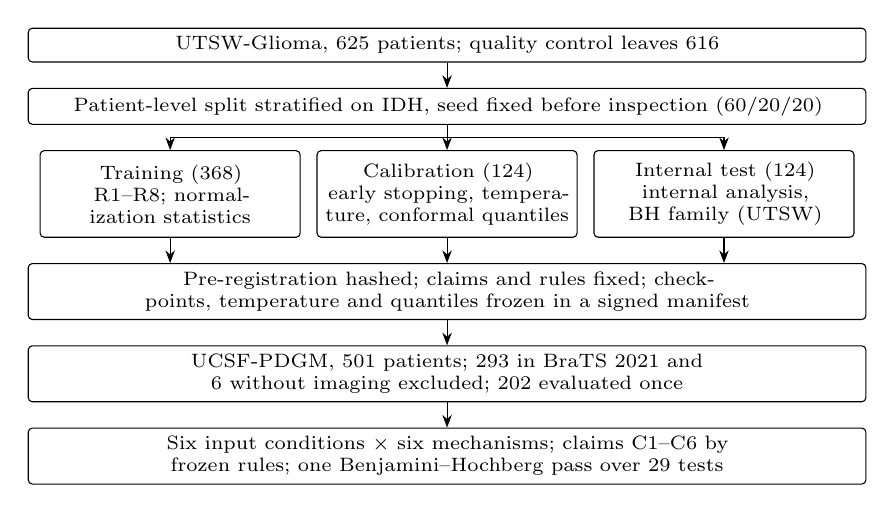
\begin{tikzpicture}[
  node distance=3.2mm,
  box/.style={draw, rounded corners=1.5pt, align=center, font=\scriptsize, inner sep=3pt, text width=0.86\columnwidth},
  half/.style={draw, rounded corners=1.5pt, align=center, font=\scriptsize, inner sep=3pt, text width=0.255\columnwidth, minimum height=11mm},
  arr/.style={-{Stealth[length=1.6mm]}, thin}]
\node[box] (utsw) {UTSW-Glioma, 625 patients; quality control leaves 616};
\node[box, below=of utsw] (split) {Patient-level split stratified on IDH, seed fixed before inspection (60/20/20)};
\node[half, below=of split] (cal) {Calibration (124)\\early stopping, temperature, conformal quantiles};
\node[half, left=2mm of cal] (train) {Training (368)\\R1--R8; normalization statistics};
\node[half, right=2mm of cal] (test) {Internal test (124)\\internal analysis, BH family (UTSW)};
\node[box, below=of cal] (freeze) {Pre-registration hashed; claims and rules fixed; checkpoints, temperature and quantiles frozen in a signed manifest};
\node[box, below=of freeze] (ucsf) {UCSF-PDGM, 501 patients; 293 in BraTS 2021 and 6 without imaging excluded; 202 evaluated once};
\node[box, below=of ucsf] (an) {Six input conditions $\times$ six mechanisms; claims C1--C6 by frozen rules; one Benjamini--Hochberg pass over $\numFamilySize$ tests};
\draw[arr] (utsw) -- (split);
\draw[arr] (split.south) -- (cal.north);
\draw[arr] (split.south) -- ++(0,-1.6mm) -| (train.north);
\draw[arr] (split.south) -- ++(0,-1.6mm) -| (test.north);
\draw[arr] (cal) -- (freeze);
\draw[arr] (train.south) -- (train.south |- freeze.north);
\draw[arr] (test.south) -- (test.south |- freeze.north);
\draw[arr] (freeze) -- (ucsf);
\draw[arr] (ucsf) -- (an);
\end{tikzpicture}
\caption{Study design. The external cohort was opened only after the freeze, and every parameter applied to it was fitted on UTSW data.}
\label{fig:design}
\end{figure}

\subsection{Cohorts}
\textbf{UTSW-Glioma} \cite{reddy2026utsw} is a public collection of 625 patients treated between 2006 and 2023, with T1, T1ce, T2, and FLAIR sequences, multilabel tumor segmentations, and molecular labels, distributed through The Cancer Imaging Archive (TCIA) \cite{clark2013}. It is not part of BraTS or TCGA, which is the main reason it serves as the development cohort. After quality control, 616 patients remained (three without an IDH label and six with a failed skull-strip check; Table~\ref{tab:flow}). IDH labels come from two assays: 413 of 622 labeled patients (66\%) by immunohistochemistry, which can miss non-R132H variants and label them wildtype, and 209 (34\%) by sequencing. Label definitions across cohorts were harmonized by one reviewer without an independent cross-check.

\textbf{UCSF-PDGM} \cite{calabrese2022ucsf} is a public collection of 501 patients scanned on a standardized 3\,T protocol. It is an external cohort that is never split or used for development. Of the 501 patients, 293 were excluded because they also appear in BraTS 2021 and 6 had no imaging, leaving $\numNExt$ patients ($\numNExtPos$ mutant, prevalence $\numPrevExt$; Table~\ref{tab:flow}). The overlap exclusion avoids patient leakage with common segmentation pre-training sets but shifts the label mix, so internal and external accuracy are not directly comparable. The assay behind UCSF-PDGM IDH labels was not independently reconfirmed against the original publication. A third cohort, the Erasmus Glioma Database (EGD) \cite{vandervoort2021egd}, is deferred to a later, separately frozen evaluation and is not part of this report.

\begin{table}[t]
\centering
\caption{Cohort Flow (Counts Only)}
\label{tab:flow}
\footnotesize
\begin{tabular}{lrr}
\toprule
Cohort & Retained & Excluded \\
\midrule
UCSF-PDGM & 202 & 299 \\
UTSW-Glioma & 616 & 9 \\
\bottomrule
\end{tabular}
%
\begin{tabular}{llr}
\toprule
Cohort & Exclusion reason & Patients \\
\midrule
UCSF-PDGM & no\_imaging\_available & 6 \\
UCSF-PDGM & overlap:brats2021 & 293 \\
UTSW-Glioma & label:idh\_unavailable & 3 \\
UTSW-Glioma & qc:skullstrip-over & 6 \\
\bottomrule
\end{tabular}

\end{table}

\subsection{Splits and Sample-Size Planning}
We split UTSW-Glioma at the patient level, stratified on IDH only, into 60/20/20 training, calibration, and internal-test sets with a seed fixed before the split was inspected. Per-class rounding gives 103 mutant and 265 wildtype patients in training (368 patients) and 35 mutant and 89 wildtype patients in each of the calibration and internal-test splits (124 each). The 1p/19q categories are reported per split but not used for stratification. A power simulation run before the split showed that at this test size the 95\% bootstrap AUROC half-width is about 0.09 at a true AUROC of 0.75 and 0.06 at 0.90 (Hanley--McNeil intervals are wider), and that no feasible calibration size on this cohort brings the coverage-deviation half-width below five percentage points, while a five-point coverage grid from 0.5 to 0.9 remains usable. The internal-test split holds $\numNIntPos$ mutant patients of $\numNInt$ (prevalence $\numPrevInt$). Split and normalization artifacts are hash-pinned and written once.

\subsection{Image Preprocessing}
For each patient the four structural sequences were rigidly registered to T1ce, skull-stripped with HD-BET \cite{isensee2019hdbet}, bias-corrected with N4 \cite{tustison2010n4}, and resampled to about 1\,mm isotropic spacing. Raw intensity scales differ widely between patients (in the training dry run the per-patient mean T1 brain intensity ranged from 123 to 271\,321 around a median of about 565, and 7\% of patients had a modality above 5\,000), so each volume was first divided by its own positive brain-voxel median. Per-modality mean and population standard deviation were then computed from the 368 training patients' brain voxels in 64-bit floating point and applied unchanged to every split and cohort. Background stays exactly zero and nothing is clipped, so external volumes need no statistics of their own. A range check found no sign of an intensity shift between the held-out UTSW splits and training.

\subsection{Network Architecture}
The classifier is a SegResNet \cite{myronenko2019segresnet} from the MONAI framework \cite{cardoso2022monai} with 32 initial filters and encoder blocks $[1,2,2,4]$, and a three-class auxiliary segmentation head (enhancing tumor, nonenhancing or necrotic core, and edema). Encoder features are pooled inside the predicted tumor region, with a fallback to global average pooling when the region is too small, and passed to a classification head with 64 hidden units and dropout 0.2. The tumor-aware pooling step follows established joint segmentation and classification designs \cite{vandervoort2023} and is confirmatory, not novel. Nothing in the architecture or training recipe was searched over; the configuration was fixed before training, and any change would have required a recorded decision.

\subsection{Training Procedure}
Table~\ref{tab:hyper} lists the fixed configuration. Training used AdamW \cite{loshchilov2019adamw} with bf16 mixed precision, gradient clipping, and deterministic kernels. The loss combined a class-weighted cross-entropy for IDH status with a Dice loss for the auxiliary segmentation. Training ran for up to 300 epochs with early stopping on the class-balanced classification loss of the calibration split, and the checkpoint with the best value was kept. Modality dropout was applied during training \cite{neverova2016}: all four sequences were kept with probability 0.5, otherwise a random nonempty subset of sequences was zeroed. Training used a single consumer GPU with 8\,GB of memory.

\begin{table}[t]
\centering
\caption{Fixed Model and Training Configuration (Not Tuned)}
\label{tab:hyper}
\footnotesize
\begin{tabular}{lp{0.52\columnwidth}}
\toprule
Setting & Value \\
\midrule
Backbone & SegResNet, 32 filters, blocks $[1,2,2,4]$ \\
Segmentation head & 3 classes, Dice loss, weight 1.0 \\
Classification head & 64 hidden units, dropout 0.2 \\
Optimizer & AdamW, lr $3\times10^{-4}$, weight decay $10^{-4}$ \\
Batch & 2, four-step gradient accumulation \\
Precision and clipping & bf16; gradient norm 1.0 \\
Epochs & up to 300; early stopping, patience 30 \\
IDH class weight & 2.57 for mutant \\
Modality dropout & all kept with probability 0.5 \\
MC dropout passes (M3) & 30 \\
Ensemble size (M4) & 5 seeds (R2--R6) \\
\bottomrule
\end{tabular}
\end{table}

\subsection{Trained Models, Ensemble, and Comparator}
Five seeds were trained (R2 to R6). R2 is the primary model, and R2 to R6 form the deep ensemble. Two pre-specified variants were trained for the confirmatory ablations: \textbf{R7}, which replaces tumor-aware pooling with global average pooling while keeping the segmentation head and loss, and \textbf{R8}, which uses two independent networks, a Dice-trained segmentation network (stage 1) and an IDH classifier (stage 2) that pools inside the frozen stage-1 mask. A comparator \textbf{R1} has the architecture of R2 but was trained without modality dropout, a joint segmentation and classification model without modality-aware training. R1 is the M6 baseline.

\subsection{Simulated Missing Sequences}
All three cohorts are curated, complete four-sequence studies, so missing sequences are simulated at inference by setting the removed channels to zero. Nothing is imputed, because imputation would mix the missing-sequence question with an imputation-quality question that this study is not designed to answer. The six conditions are complete input, removal of each of T1, T1ce, T2, and FLAIR, and T1ce+FLAIR only, the last a common abbreviated protocol. Every table and figure that involves a removed sequence is labeled ``simulated'' (abbreviated ``sim.'').

\subsection{Abstention Mechanisms}
Each mechanism assigns a confidence $\kappa$ to every patient, and the model abstains on the least confident cases.
\begin{itemize}[leftmargin=1.2em]
\item \textbf{M1} uses $\kappa=\max(\hat p,1-\hat p)$ of the raw probability of mutation, the binary form of the maximum softmax probability \cite{hendrycks2017}.
\item \textbf{M2} uses the same score on the temperature-scaled probability $\hat p_T=\sigma(z/T)$, where $z$ is the logit \cite{guo2017}. The temperature $T=\numTemperature$ was fitted once by minimizing the binary cross-entropy on the UTSW calibration split of the primary model and was never refitted on any other data.
\item \textbf{M3} uses the negative predictive entropy of $\bar p=\frac{1}{30}\sum_{k=1}^{30}\hat p^{(k)}$ over 30 Monte Carlo passes through the dropout layer of the classification head \cite{gal2016}, the only dropout layer in the model: $\kappa=\bar p\log\bar p+(1-\bar p)\log(1-\bar p)$.
\item \textbf{M4} uses the negative population variance of the five ensemble members' probabilities \cite{lakshminarayanan2017}, $\kappa=-\frac15\sum_{j=1}^{5}(\hat p_j-\bar p)^2$, which ranks by disagreement only.
\item \textbf{M5} is split conformal prediction (Fig.~\ref{fig:alg}). The score-threshold view ranks by $\max(\hat p_T,1-\hat p_T)$. The set-valued view uses the nonconformity score and quantile rule of Section~\ref{sec:formal} for $\alpha\in\{0.05,0.1,0.2\}$, with the calibration quantiles carried over unchanged to every condition and cohort.
\item \textbf{M6} is the comparator R1 with raw confidence and no temperature.
\end{itemize}
Because temperature scaling is monotone, M1, M2, and M5 rank patients identically; they differ in operating points and in set-valued coverage. A random-confidence control, the same losses under a random ordering, was computed as a reference. As a diagnostic we also report a \emph{refit} variant that recomputes the quantile on the calibration split in each condition; the frozen method is the carried-over variant. For the 0--1 loss, M1, M2, M3, and M5 use the error of the raw single-model classifier ($\hat p\ge0.5$), and M4 uses the error of the ensemble-mean classifier, so its always-predict risk can differ slightly.

\subsection{Evaluation Metrics}
Selective risk is evaluated at $\phi\in\{0.5,0.6,0.7,0.8,0.9\}$, and the attained coverage is reported. AURC and the oracle AURC follow \eqref{eq:aurc}. Calibration uses \eqref{eq:ece} and the Brier score. Discrimination uses the AUROC with the Hanley--McNeil interval \cite{hanley1982}, the wider of the two intervals we compute, and a bootstrap interval, together with the area under the precision--recall curve. AUROC is never reported without ECE, Brier score, AURC, and coverage beside it. Coverage deviation \eqref{eq:covdev} has the two-stage bootstrap interval of Fig.~\ref{fig:alg}. We label a deviation \emph{preserved} if its interval lies inside $\pm0.07$, \emph{degraded} if it lies wholly outside, and \emph{indeterminate} otherwise; the $\pm0.05$ band is a secondary reading.

\subsection{Pre-Registered Claims and Decision Rules}
\label{sec:claims}
Six claims were fixed before any external result was seen (Table~\ref{tab:claimdefs}). If neither the refutation nor the support rule applies, the claim is \emph{inconclusive at this sample size}. The worst status over conditions decides a claim. For C6 the enrichment is \eqref{eq:enrich}, and the one-sided permutation test shuffles the loss vector. Refutations are reported as refutations, and the rules were not changed after any result.

\begin{table*}[t]
\centering
\caption{Pre-Registered Claims and Frozen Decision Rules. $D(\phi)$ Is the Selective Minus the Always-Predict Risk at Coverage $\phi$}
\label{tab:claimdefs}
\footnotesize
\begin{tabular}{p{0.8cm}p{5.4cm}p{4.6cm}p{4.6cm}}
\toprule
Claim & Statement & Refuted if & Supported if \\
\midrule
C1 & Conformal selective prediction has lower selective risk than always predicting, internally (complete input). & Any point estimate of $D(\phi)\ge0$. & Every upper 95\% limit of $D(\phi)<0$. \\
C2 & The advantage survives missing sequences. & As C1, per condition. & As C1, per condition. \\
C3 & The advantage survives external shift. & As C1 on the external cohort (complete input; missing-sequence conditions secondary). & As C1 on the external cohort. \\
C4 & Coverage deviation can be characterized within the pre-registered tolerance. & Any condition's deviation interval has half-width $>0.07$. & Every half-width $\le0.07$. \\
C5 & Risk--coverage curves are monotone. & Any adjacent-coverage lower 95\% limit $>0$ (risk at lower coverage minus risk at higher). & Every adjacent point difference $\le0$. \\
C6 & Abstention is enriched for errors. & Any observed enrichment $\le0$. & Every BH-adjusted one-sided permutation $p<0.05$ across the five coverages. \\
\bottomrule
\end{tabular}
\end{table*}

\subsection{Statistical Analysis}
Intervals use $B=\numBootDraws$ bootstrap draws over patients \cite{efron1979} with one shared patient-index matrix per cohort, so that paired comparisons use the same resamples, and percentile limits. Permutation tests use $\numPermDraws$ draws with
\begin{equation}
p=\frac{1+\#\{b:\ T^{(b)}\ \text{at least as extreme as}\ T\}}{B+1}.
\end{equation}
AUROC differences use the DeLong test \cite{delong1988}. The confirmatory family has $\numFamilySize$ comparisons, 14 on UTSW and 15 on UCSF-PDGM, in five blocks: (A) mechanism contrasts at complete input; (B) each missing-sequence condition against complete input; (C) external against internal AURC, unpaired; (D) raw against temperature-scaled calibration; and (E) the ablations R7 and R8 against R2. They were adjusted once with the Benjamini--Hochberg procedure \cite{benjamini1995}: with ordered raw values $p_{(1)}\le\dots\le p_{(m)}$, the adjusted value is
\begin{equation}
\tilde p_{(k)}=\min_{j\ge k}\min\!\left(1,\frac{m\,p_{(j)}}{j}\right),
\end{equation}
and a test is rejected if $\tilde p\le q=0.05$. The pre-registered family was 44 comparisons with EGD and 29 without; EGD is deferred, so the family is 29. Claims C1 to C6 follow their own decision rules and sit outside the family.

\subsection{Protocol Integrity and Independent Verification}
\label{sec:integrity}
External predictions were produced once by a harness that refuses to run without a signed freeze manifest naming the exact checkpoints, calibration parameters (temperature and conformal quantiles, fitted on the UTSW calibration split only), and code commit, that checks every input hash, and that rechecks the repository state after the run. A firewall in the evaluation code prevents any metric from being computed against external labels unless the evaluation is authorized. Per-patient predictions were written to hash-checked files, and the external analysis code was written and tested on synthetic data before it saw any real external prediction. The first manifest omitted R7 and R8; this was found before any external metric was examined and corrected with a second signed manifest and a second run, with no change to any method (Appendix~\ref{app:deviations}).

The external numbers were independently recomputed by a second software agent working from the written metric contracts and the frozen prediction files, without access to the analysis code or results; its results file was written before any comparison. Section~\ref{sec:verification} reports the outcome.

\subsection{Software and Compute}
The pipeline uses Python with PyTorch and MONAI \cite{cardoso2022monai}. Inference for the external cohort ran on the same single consumer GPU as training. Statistical analysis and manuscript generation ran on a CPU. All numbers in this manuscript are inserted by scripts that read the frozen result files (Appendix~\ref{app:repro}).

\section{Results}
\label{sec:results}

\subsection{Cohorts}
The internal test split held $\numNInt$ patients ($\numNIntPos$ mutant, prevalence $\numPrevInt$) and the external cohort $\numNExt$ patients ($\numNExtPos$ mutant, prevalence $\numPrevExt$) after the exclusions in Table~\ref{tab:flow}. Every cohort--condition--mechanism cell for UTSW and UCSF-PDGM is present.

\subsection{Discrimination and Calibration on Complete Input}
On the internal test split the primary model reached an AUROC of \numIntRTwoAuroc{} (95\% interval \numIntAurocLo{} to \numIntAurocHi{}) and on UCSF-PDGM \numExtRTwoAuroc{} (\numExtAurocLo{} to \numExtAurocHi{}; Table~\ref{tab:main}). The external value is higher. Prevalence differs and the external cohort was filtered for BraTS overlap, so we do not read this as better generalization.

\begin{table}[t]
\centering
\caption{Primary Model and Ablations on Complete Input (Temperature-Scaled ECE and Brier Score; AURC as Mean Over Cutoffs)}
\label{tab:main}
\footnotesize
\begin{tabular}{llcccc}
\toprule
Cohort & Model & AUROC & ECE & Brier & AURC \\
\midrule
UTSW test & R2 & \numIntRTwoAuroc & \numIntRTwoEce & \numIntRTwoBrier & \numIntRTwoAurc \\
UTSW test & R7 & \numIntRSevenAuroc & \numIntRSevenEce & \numIntRSevenBrier & \numIntRSevenAurc \\
UTSW test & R8 & \numIntREightAuroc & \numIntREightEce & \numIntREightBrier & \numIntREightAurc \\
UCSF-PDGM & R2 & \numExtRTwoAuroc & \numExtRTwoEce & \numExtRTwoBrier & \numExtRTwoAurc \\
UCSF-PDGM & R7 & \numExtRSevenAuroc & \numExtRSevenEce & \numExtRSevenBrier & \numExtRSevenAurc \\
UCSF-PDGM & R8 & \numExtREightAuroc & \numExtREightEce & \numExtREightBrier & \numExtREightAurc \\
\bottomrule
\end{tabular}
\end{table}

\subsection{Calibration Across Cohorts (RQ3)}
Temperature-scaled ECE was \numIntEceMTwo{} (bootstrap interval \numIntEceMTwoLo{} to \numIntEceMTwoHi{}) internally and \numExtEceMTwo{} (\numExtEceMTwoLo{} to \numExtEceMTwoHi{}) externally; the Brier score was \numIntBrierMTwo{} and \numExtBrierMTwo{}. We found no degradation from internal to external data, and the intervals overlap. No family test addresses this contrast, so the statement is descriptive. Temperature scaling did not lower ECE on either cohort (raw ECE \numIntEceMOne{} internally and \numExtEceMOne{} externally, raw Brier score \numIntBrierMOne{} and \numExtBrierMOne{}), and the fitted temperature was close to one ($T=\numTemperature$), so the raw network was already close to calibrated on the calibration split. The raw Brier score on UCSF-PDGM was lower than the scaled one by \numExtDTwoAbs{}, a difference that is statistically detectable (adjusted $p=\numFamXDTwoAdj$) and clinically negligible.

Fig.~\ref{fig:rel} shows the internal reliability diagrams for each condition. On complete input and under most single-sequence removals the binned observed fractions follow the diagonal loosely, mostly at or below it in the upper bins, with the scatter expected from bins that hold few patients. With T1ce removed the diagram flattens: for predicted probabilities above one half the observed fraction of mutant patients stays well below the prediction, and both the raw and the scaled curves leave the diagonal. Temperature scaling, a single parameter fitted on complete input, cannot correct that pattern.

\begin{figure*}[t]
\centering
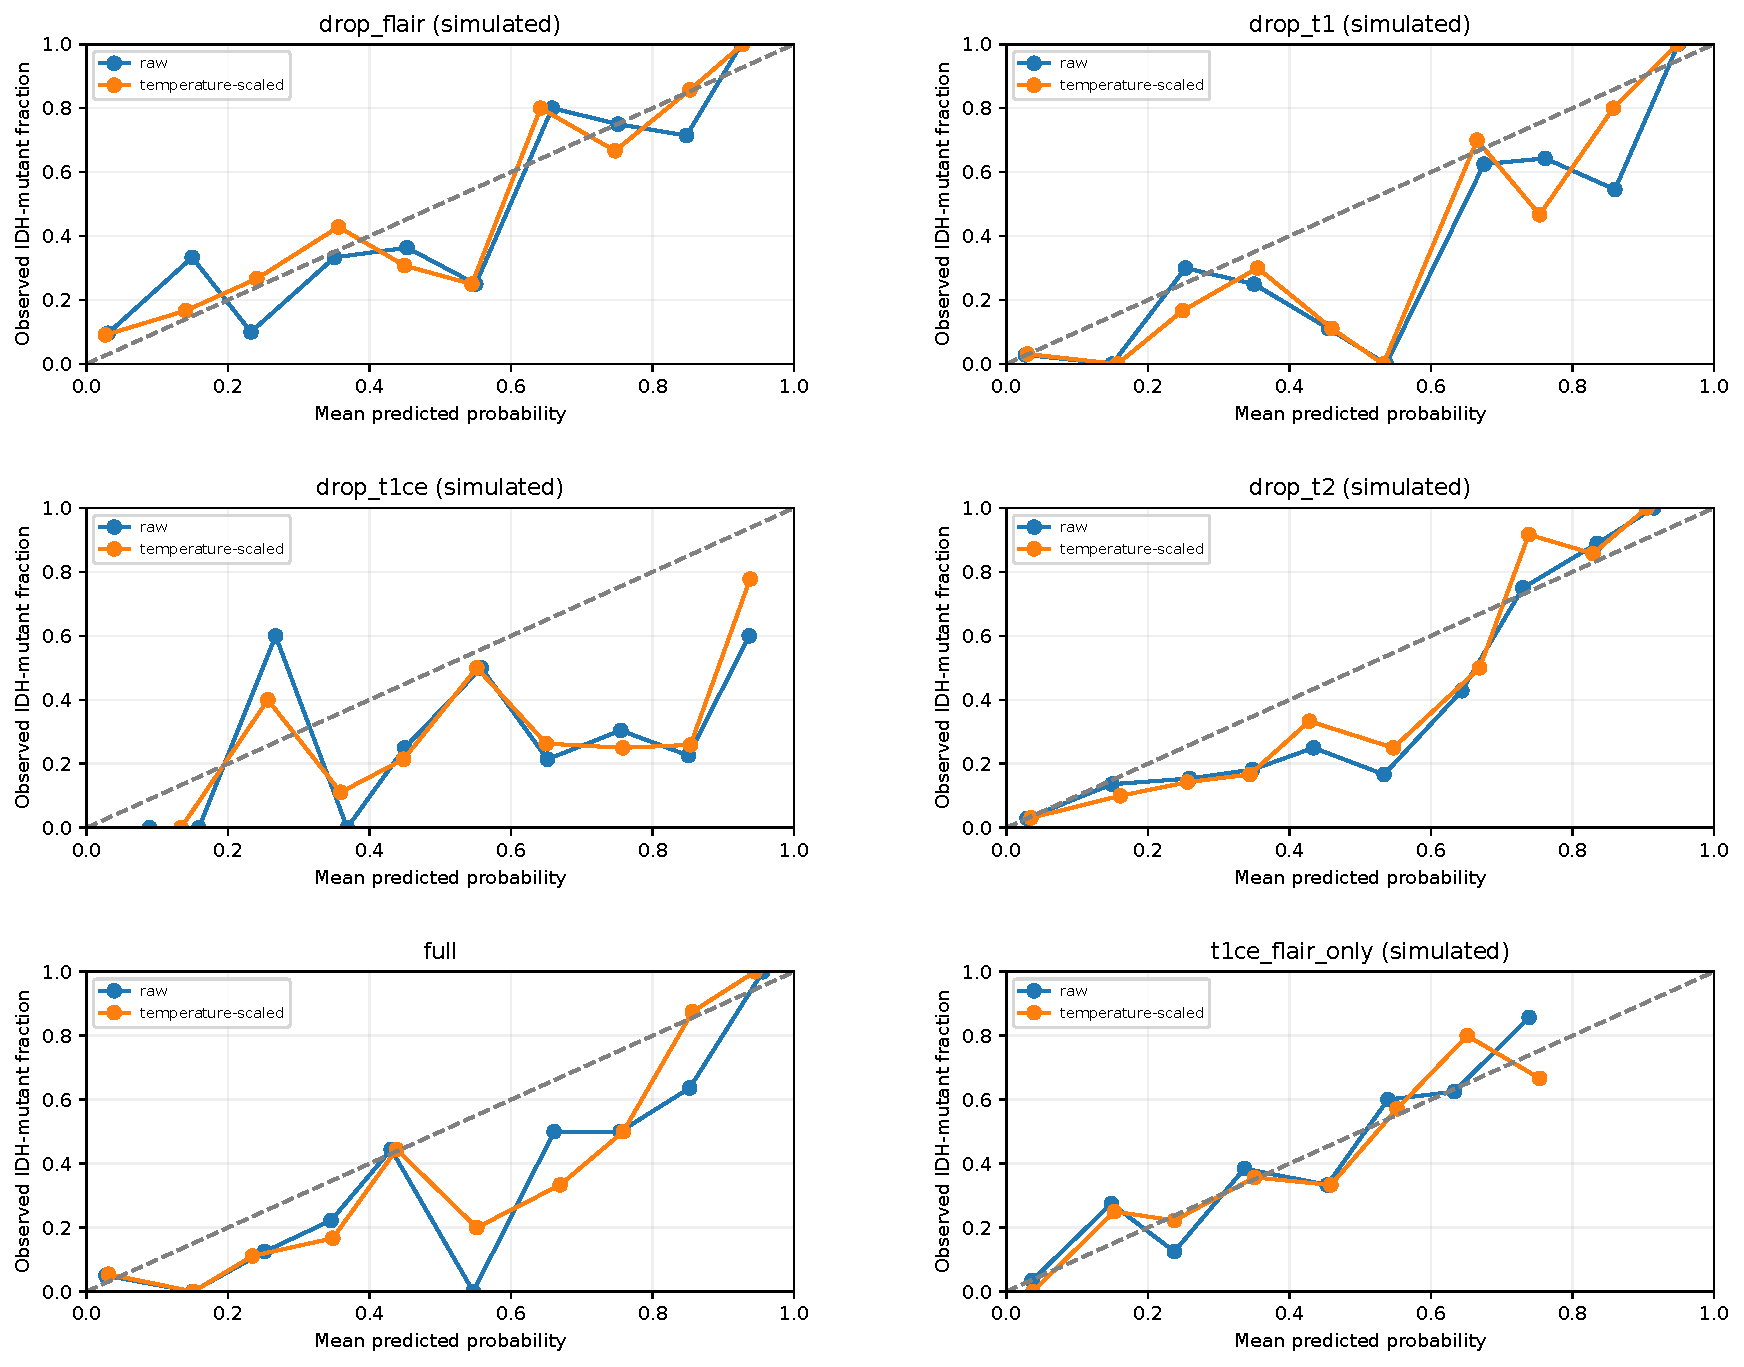
\includegraphics[width=0.78\textwidth]{figures/journal_fig_rel_utsw.pdf}
\caption{Reliability diagrams on the UTSW internal test split for each input condition, raw and temperature-scaled probabilities, ten equal-width bins (empty bins not drawn). The temperature is the frozen value fitted on complete input. Missing-sequence conditions are simulated.}
\label{fig:rel}
\end{figure*}

\subsection{Does Abstaining Lower Risk? (RQ1, C1, C3)}
Table~\ref{tab:risk} gives the selective risk at each target coverage with its interval, and Figs.~\ref{fig:rcint} and~\ref{fig:rc} show the curves. Internally the always-predict risk was \numIntAlwaysFull{} and the selective risk fell to \numIntRiskZeroFive{} at coverage 0.5; externally the always-predict risk was \numExtAlwaysFull{} and the selective risk fell to \numExtRiskZeroFive{}. On complete input every upper 95\% limit of $D(\phi)$ was below zero on both cohorts, so C1 is supported and C3 is supported on complete input (external $D$ of \numCThreeDeltaZeroNine{} at coverage 0.9 and \numCThreeDeltaZeroFive{} at 0.5, with upper limits \numCThreeUpperZeroNine{} and \numCThreeUpperZeroFive{}). Internally $D(\phi)$ on complete input was \numCOneDeltaZeroNine{} at coverage 0.9 and \numCOneDeltaZeroFive{} at 0.5. The oracle AURC, the lowest value any ordering of the same predictions can reach, was \numIntOracle{} internally and \numExtOracle{} externally, against observed AURCs of \numIntAurcFull{} and \numExtAurcFull{}, so the confidence ranking is useful but leaves room for a better one.

\begin{table*}[t]
\centering
\caption{Selective Risk of the Primary Model (M2) at Target Coverage, 95\% Bootstrap Interval in Brackets. Missing-Sequence Conditions Are Simulated}
\label{tab:risk}
\footnotesize
\textbf{UTSW internal test} \\[2pt]
\begin{tabular}{lccccc}
\toprule
Condition & 0.5 & 0.6 & 0.7 & 0.8 & 0.9 \\
\midrule
Full & 0.048 [0.000, 0.127] & 0.093 [0.026, 0.173] & 0.115 [0.056, 0.205] & 0.160 [0.080, 0.240] & 0.170 [0.107, 0.259] \\
$-$T1 (sim.) & 0.048 [0.000, 0.127] & 0.093 [0.027, 0.187] & 0.126 [0.057, 0.207] & 0.150 [0.080, 0.230] & 0.161 [0.098, 0.241] \\
$-$T1ce (sim.) & 0.548 [0.429, 0.677] & 0.587 [0.474, 0.693] & 0.598 [0.494, 0.701] & 0.580 [0.480, 0.683] & 0.545 [0.455, 0.634] \\
$-$T2 (sim.) & 0.081 [0.016, 0.145] & 0.080 [0.026, 0.147] & 0.092 [0.034, 0.170] & 0.130 [0.070, 0.208] & 0.134 [0.080, 0.221] \\
$-$FLAIR (sim.) & 0.081 [0.032, 0.177] & 0.133 [0.053, 0.227] & 0.149 [0.080, 0.230] & 0.180 [0.100, 0.248] & 0.188 [0.124, 0.277] \\
T1ce+FLAIR (sim.) & 0.161 [0.065, 0.254] & 0.160 [0.080, 0.250] & 0.172 [0.080, 0.250] & 0.180 [0.109, 0.267] & 0.196 [0.133, 0.281] \\
\bottomrule
\end{tabular}
 \\[6pt]
\textbf{UCSF-PDGM external} \\[2pt]
\begin{tabular}{lccccc}
\toprule
Condition & 0.5 & 0.6 & 0.7 & 0.8 & 0.9 \\
\midrule
Full & 0.030 [0.000, 0.089] & 0.066 [0.025, 0.115] & 0.085 [0.035, 0.134] & 0.111 [0.062, 0.166] & 0.126 [0.077, 0.181] \\
$-$T1 (sim.) & 0.050 [0.010, 0.099] & 0.066 [0.025, 0.115] & 0.077 [0.042, 0.134] & 0.111 [0.062, 0.167] & 0.148 [0.093, 0.203] \\
$-$T1ce (sim.) & 0.317 [0.218, 0.396] & 0.344 [0.252, 0.436] & 0.394 [0.310, 0.486] & 0.444 [0.368, 0.521] & 0.445 [0.377, 0.516] \\
$-$T2 (sim.) & 0.020 [0.000, 0.059] & 0.025 [0.000, 0.074] & 0.070 [0.021, 0.119] & 0.080 [0.043, 0.134] & 0.110 [0.060, 0.159] \\
$-$FLAIR (sim.) & 0.099 [0.049, 0.168] & 0.115 [0.057, 0.179] & 0.148 [0.085, 0.204] & 0.160 [0.104, 0.216] & 0.181 [0.121, 0.236] \\
T1ce+FLAIR (sim.) & 0.020 [0.000, 0.097] & 0.066 [0.025, 0.123] & 0.099 [0.049, 0.162] & 0.130 [0.074, 0.191] & 0.165 [0.109, 0.219] \\
\bottomrule
\end{tabular}

\end{table*}

\begin{figure*}[t]
\centering
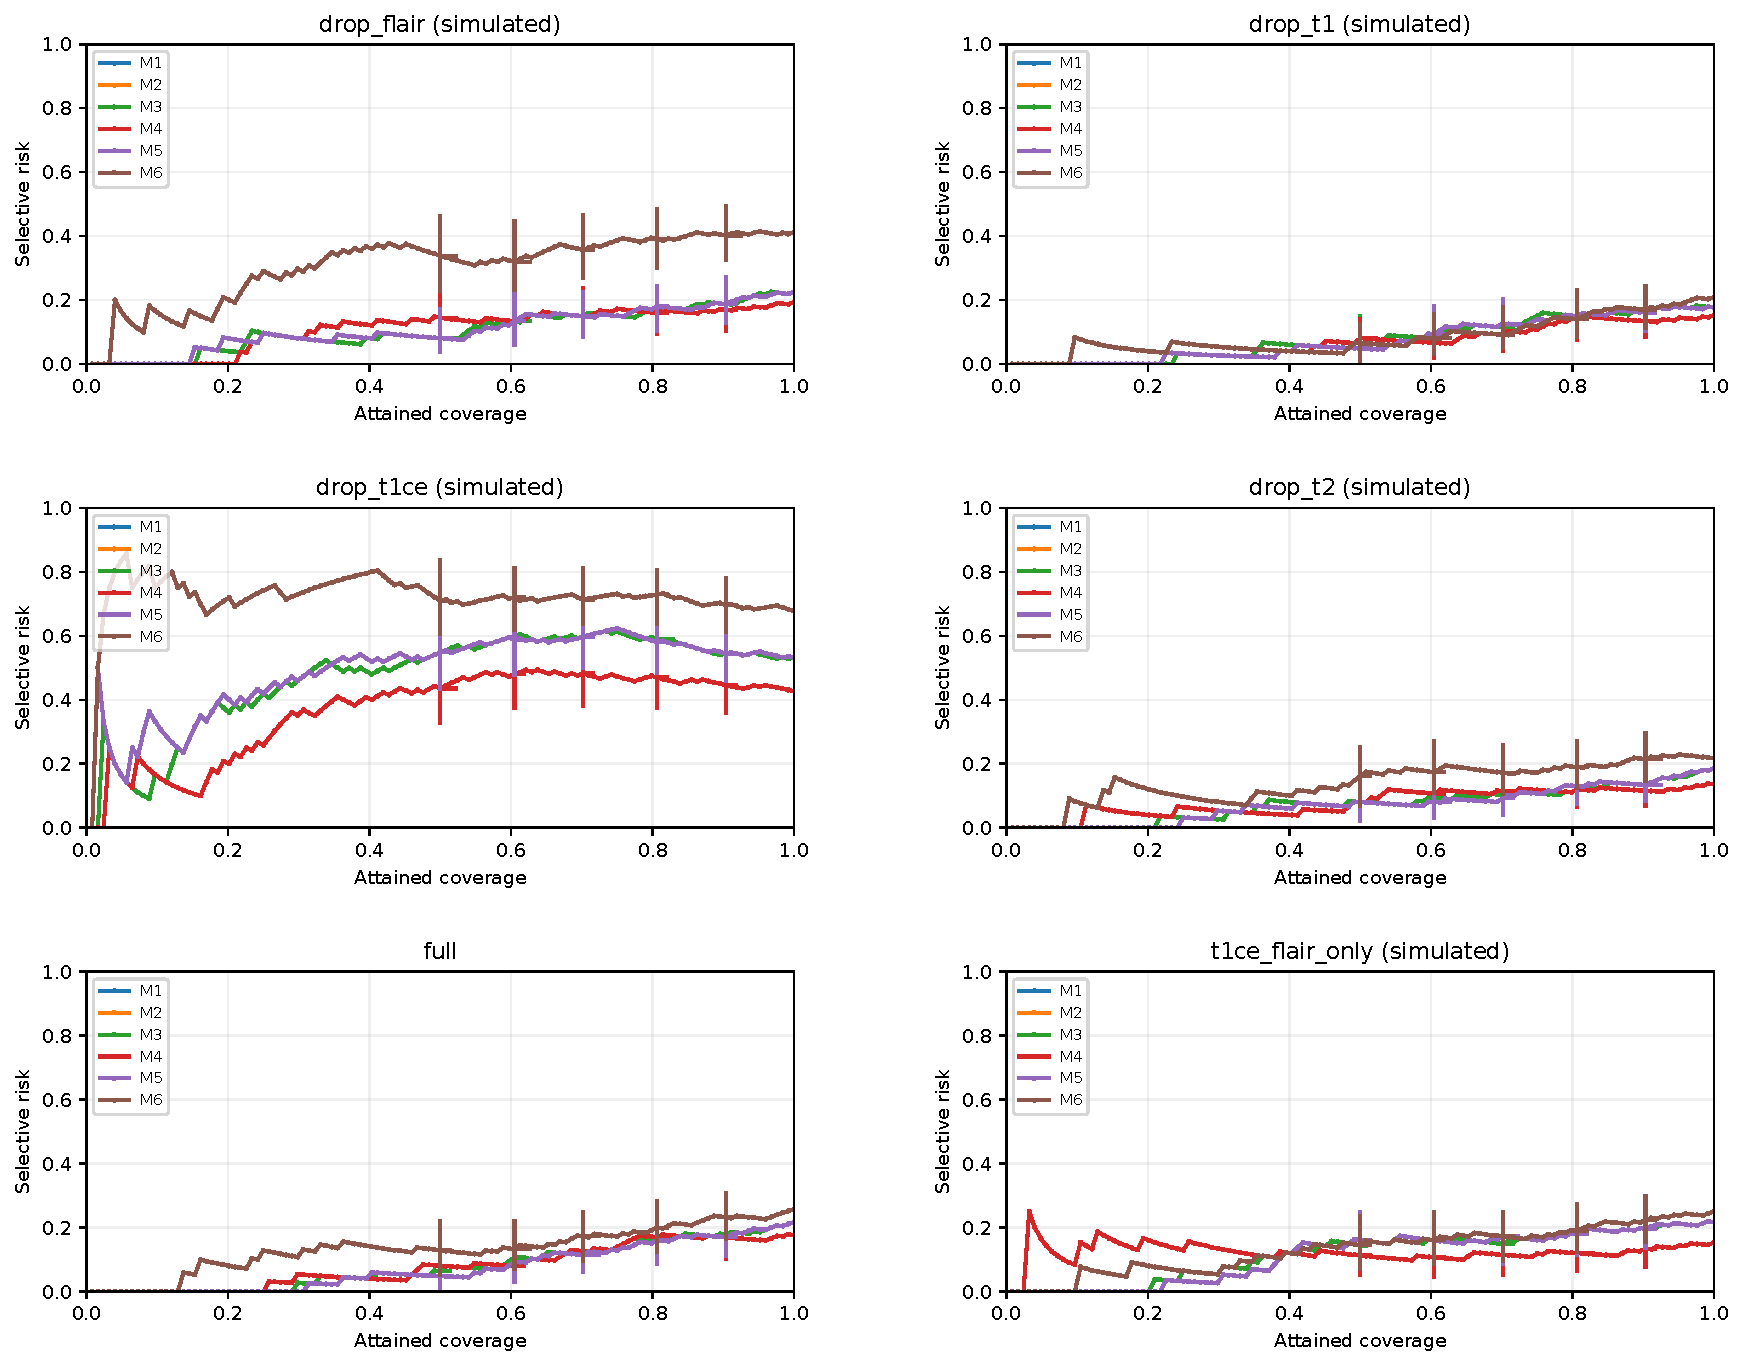
\includegraphics[width=0.80\textwidth]{figures/journal_fig_rc_utsw.pdf}
\caption{Risk--coverage curves on the UTSW internal test split for each input condition and mechanisms M1 to M6. Vertical bars are 95\% intervals at the five evaluated coverage levels. Missing-sequence conditions are simulated.}
\label{fig:rcint}
\end{figure*}

\begin{figure*}[t]
\centering
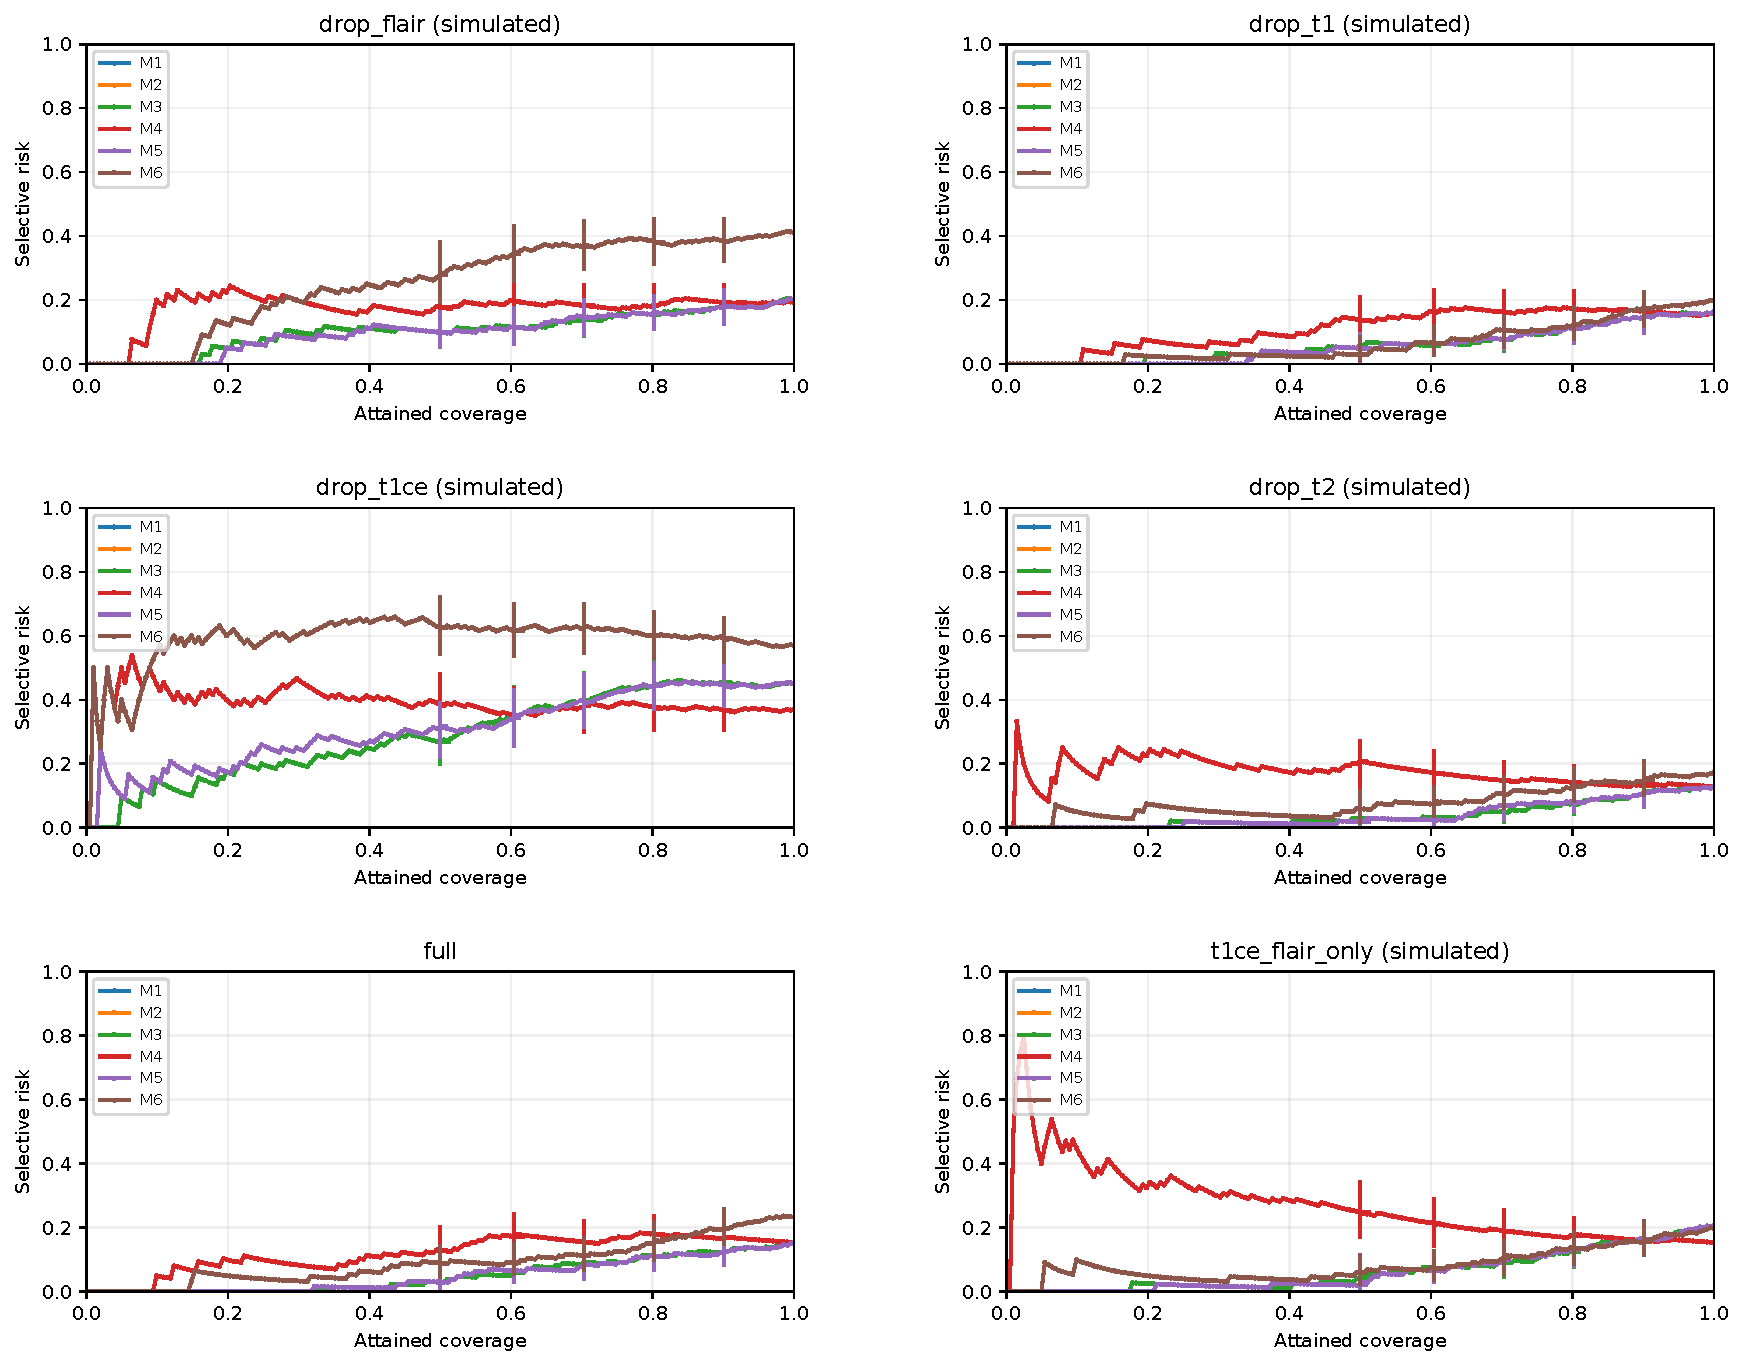
\includegraphics[width=0.80\textwidth]{figures/journal_fig_rc_ucsf.pdf}
\caption{Risk--coverage curves on UCSF-PDGM for each input condition and mechanisms M1 to M6. Vertical bars are 95\% intervals at the five evaluated coverage levels. Missing-sequence conditions are simulated.}
\label{fig:rc}
\end{figure*}

\subsection{Comparing Abstention Mechanisms}
Table~\ref{tab:aurc} lists the AURC for every mechanism and condition. On complete input the mechanisms differ little: internally M1, M2, and M5 reached \numIntAurcMTwoFull{}, M3 \numIntAurcMThreeFull{}, and M4 \numIntAurcMFourFull{}; externally \numExtAurcMTwoFull{}, \numExtAurcMThreeFull{}, and \numExtAurcMFourFull{}. The contrast of the conformal ranking with MC dropout was not different from zero after adjustment (UCSF-PDGM adjusted $p=\numFamXAOneAdj$). The ensemble-variance ranking was worse than the confidence ranking on UCSF-PDGM (adjusted $p=\numFamXATwoAdj$), and so was its contrast with MC dropout (adjusted $p=\numFamXAThreeAdj$). On UTSW none of the three block-A contrasts was rejected (adjusted $p=\numFamUAOneAdj$, \numFamUATwoAdj, and \numFamUAThreeAdj). The comparator without modality dropout (M6) was worse than the primary model on complete input (\numIntAurcMSixFull{} internally, \numExtAurcMSixFull{} externally) and much worse with T1ce removed (\numIntAurcMSixDropTonece{} internally, \numExtAurcMSixDropTonece{} externally). Conformal prediction therefore adds no ranking advantage over temperature-scaled confidence; its contribution is a coverage target, examined below.

\begin{table*}[t]
\centering
\caption{AURC (Mean Over Cutoffs) by Mechanism and Condition, With Always-Predict Risk and Oracle AURC. M6 Is the No-Modality-Dropout Comparator. Missing-Sequence Conditions Are Simulated}
\label{tab:aurc}
\footnotesize
\textbf{UTSW internal test} \\[2pt]
\begin{tabular}{lrrrrrrrr}
\toprule
Condition & Always & Oracle & M1 & M2 & M3 & M4 & M5 & M6 \\
\midrule
Full & 0.218 & 0.027 & 0.076 & 0.076 & 0.080 & 0.080 & 0.076 & 0.134 \\
$-$T1 (sim.) & 0.177 & 0.017 & 0.076 & 0.076 & 0.080 & 0.071 & 0.076 & 0.085 \\
$-$T1ce (sim.) & 0.532 & 0.179 & 0.493 & 0.493 & 0.473 & 0.370 & 0.493 & 0.723 \\
$-$T2 (sim.) & 0.185 & 0.019 & 0.073 & 0.073 & 0.075 & 0.079 & 0.073 & 0.141 \\
$-$FLAIR (sim.) & 0.226 & 0.029 & 0.108 & 0.108 & 0.106 & 0.112 & 0.108 & 0.308 \\
T1ce+FLAIR (sim.) & 0.218 & 0.027 & 0.113 & 0.113 & 0.117 & 0.124 & 0.113 & 0.133 \\
\bottomrule
\end{tabular}
 \\[6pt]
\textbf{UCSF-PDGM external} \\[2pt]
\begin{tabular}{lrrrrrrrr}
\toprule
Condition & Always & Oracle & M1 & M2 & M3 & M4 & M5 & M6 \\
\midrule
Full & 0.153 & 0.013 & 0.051 & 0.051 & 0.051 & 0.120 & 0.051 & 0.092 \\
$-$T1 (sim.) & 0.163 & 0.015 & 0.058 & 0.058 & 0.061 & 0.112 & 0.058 & 0.065 \\
$-$T1ce (sim.) & 0.450 & 0.123 & 0.310 & 0.310 & 0.290 & 0.393 & 0.310 & 0.589 \\
$-$T2 (sim.) & 0.129 & 0.009 & 0.040 & 0.040 & 0.039 & 0.173 & 0.040 & 0.078 \\
$-$FLAIR (sim.) & 0.203 & 0.023 & 0.101 & 0.101 & 0.105 & 0.175 & 0.101 & 0.255 \\
T1ce+FLAIR (sim.) & 0.208 & 0.024 & 0.064 & 0.064 & 0.065 & 0.270 & 0.064 & 0.083 \\
\bottomrule
\end{tabular}

\end{table*}

\subsection{Missing Sequences (RQ1, C2)}
Removing T1ce had the largest effect. Internally, with T1ce removed, the AURC of the primary model was \numIntAurcMTwoDropTonece{} against an always-predict risk of \numIntAlwaysDropTonece{}, and $D(\phi)$ was positive at every coverage level from 0.5 to 0.9 (Table~\ref{tab:deltaint} in Appendix~\ref{app:tables}), so C2 is refuted. The external AURC with T1ce removed was \numExtAurcMTwoDropTonece{} against \numExtAlwaysDropTonece{}, and its increase over complete input is one of the rejected family members on both cohorts (internal adjusted $p=\numFamUBTwoAdj$, external $p=\numFamXBTwoAdj$). Removing FLAIR also raised the external AURC, by less (adjusted $p=\numFamXBFourAdj$; internal $p=\numFamUBFourAdj$). Removing T1 or T2 changed little on either cohort (internal adjusted $p=\numFamUBOneAdj$ and \numFamUBThreeAdj{}; external \numFamXBOneAdj{} and \numFamXBThreeAdj{}), and neither did reducing the input to T1ce and FLAIR (internal \numFamUBFiveAdj{}, external \numFamXBFiveAdj{}). The ensemble-variance score (M4) ranked errors better than the confidence score with T1ce removed internally (AURC \numIntAurcMFourDropTonece{} against \numIntAurcMTwoDropTonece{}), but not externally (\numExtAurcMFourDropTonece{} against \numExtAurcMTwoDropTonece{}); this contrast was not in the confirmatory family and is descriptive.

\subsection{Monotonicity (C5)}
Table~\ref{tab:mono} in Appendix~\ref{app:tables} reports the adjacent-coverage risk differences. Risk--coverage curves were monotone on the five-point grid in every external condition, with every adjacent point difference at or below zero, so C5 is supported externally. Internally C5 is inconclusive: the point differences are not all nonpositive, and some intervals include positive values. The curves are not monotone at the finest scale, where the number of violating adjacent cutoff pairs is nonzero in every condition; C5 is defined on the five-point grid, which is where the pre-registered rule applies.

\subsection{Is Abstention Enriched for Errors? (C6)}
Externally, the abstained cases had a higher error rate than the cohort average at every coverage level in every condition, and the BH-adjusted permutation $p$ was below 0.05 in four of six conditions. The two exceptions (T1 removed and T1ce removed) are inconclusive, so the external claim is \numStatusCSixExt. Internally, with T1ce removed, the observed enrichment was at or below zero at every coverage level, so C6 is refuted internally (Table~\ref{tab:enrichint}). In that condition the least confident cases of the model were no more likely to be wrong than a random subset.

Figs.~\ref{fig:abstint} and~\ref{fig:abst} show the cost side: the fraction of rejected patients who would have been classified correctly. For the confidence-based mechanisms on complete input, more than half of the rejected patients would have been classified correctly at most operating points, and the rate falls as coverage rises, because the patients rejected at high coverage are the least confident. For the ensemble-variance score it is higher in most conditions, which matches its weaker AURC: disagreement among members rejects many patients whom every member classifies correctly. With T1ce removed the confidence-based rate is lower at coverage 0.5 on both cohorts, but only because the model is wrong on many more patients, not because the ranking is better.

\begin{figure*}[t]
\centering
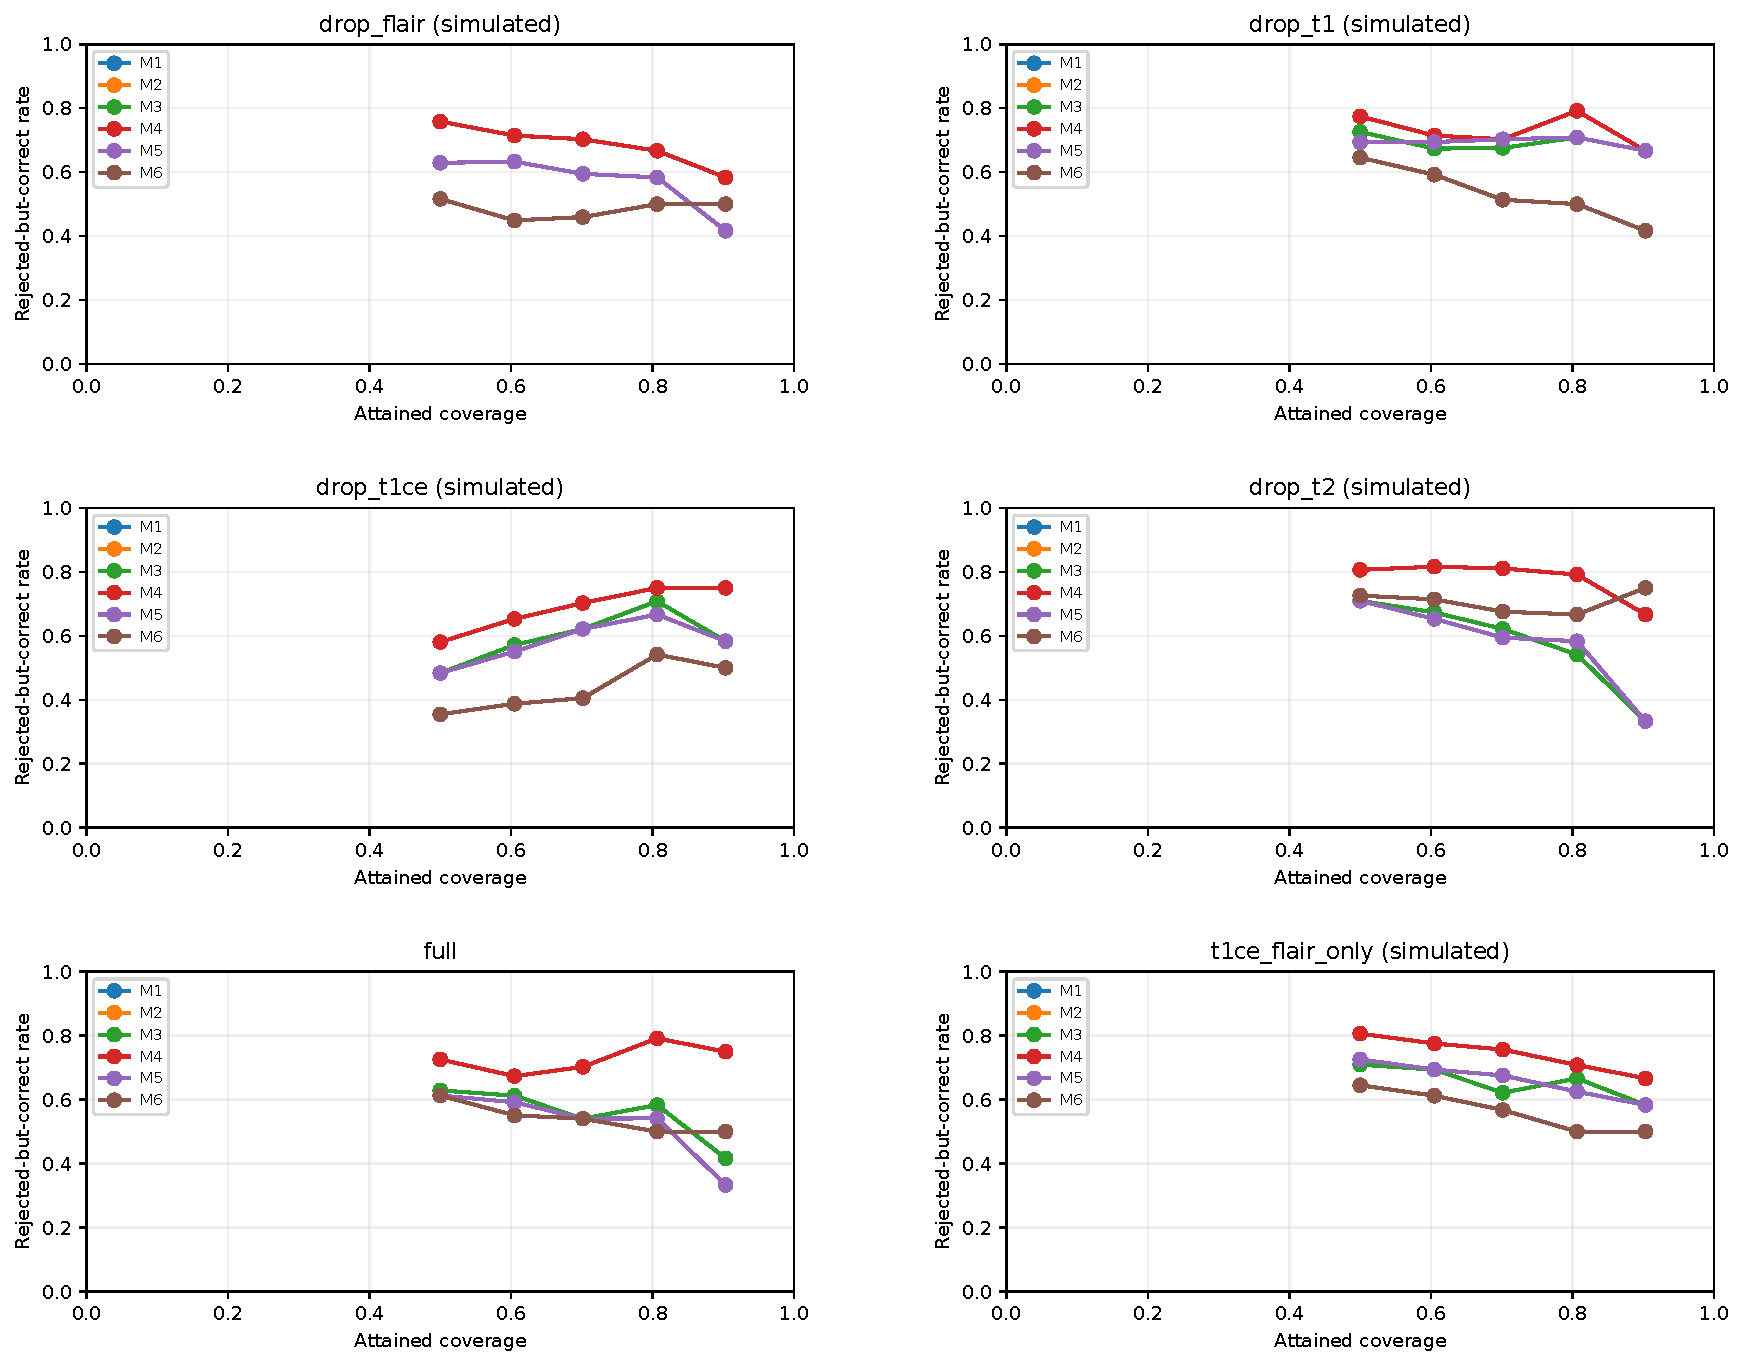
\includegraphics[width=0.78\textwidth]{figures/journal_fig_abst_utsw.pdf}
\caption{Rejected-but-correct rate against attained coverage on the UTSW internal test split, by condition and mechanism. No intervals are stored for this rate. Missing-sequence conditions are simulated.}
\label{fig:abstint}
\end{figure*}

\begin{figure*}[t]
\centering
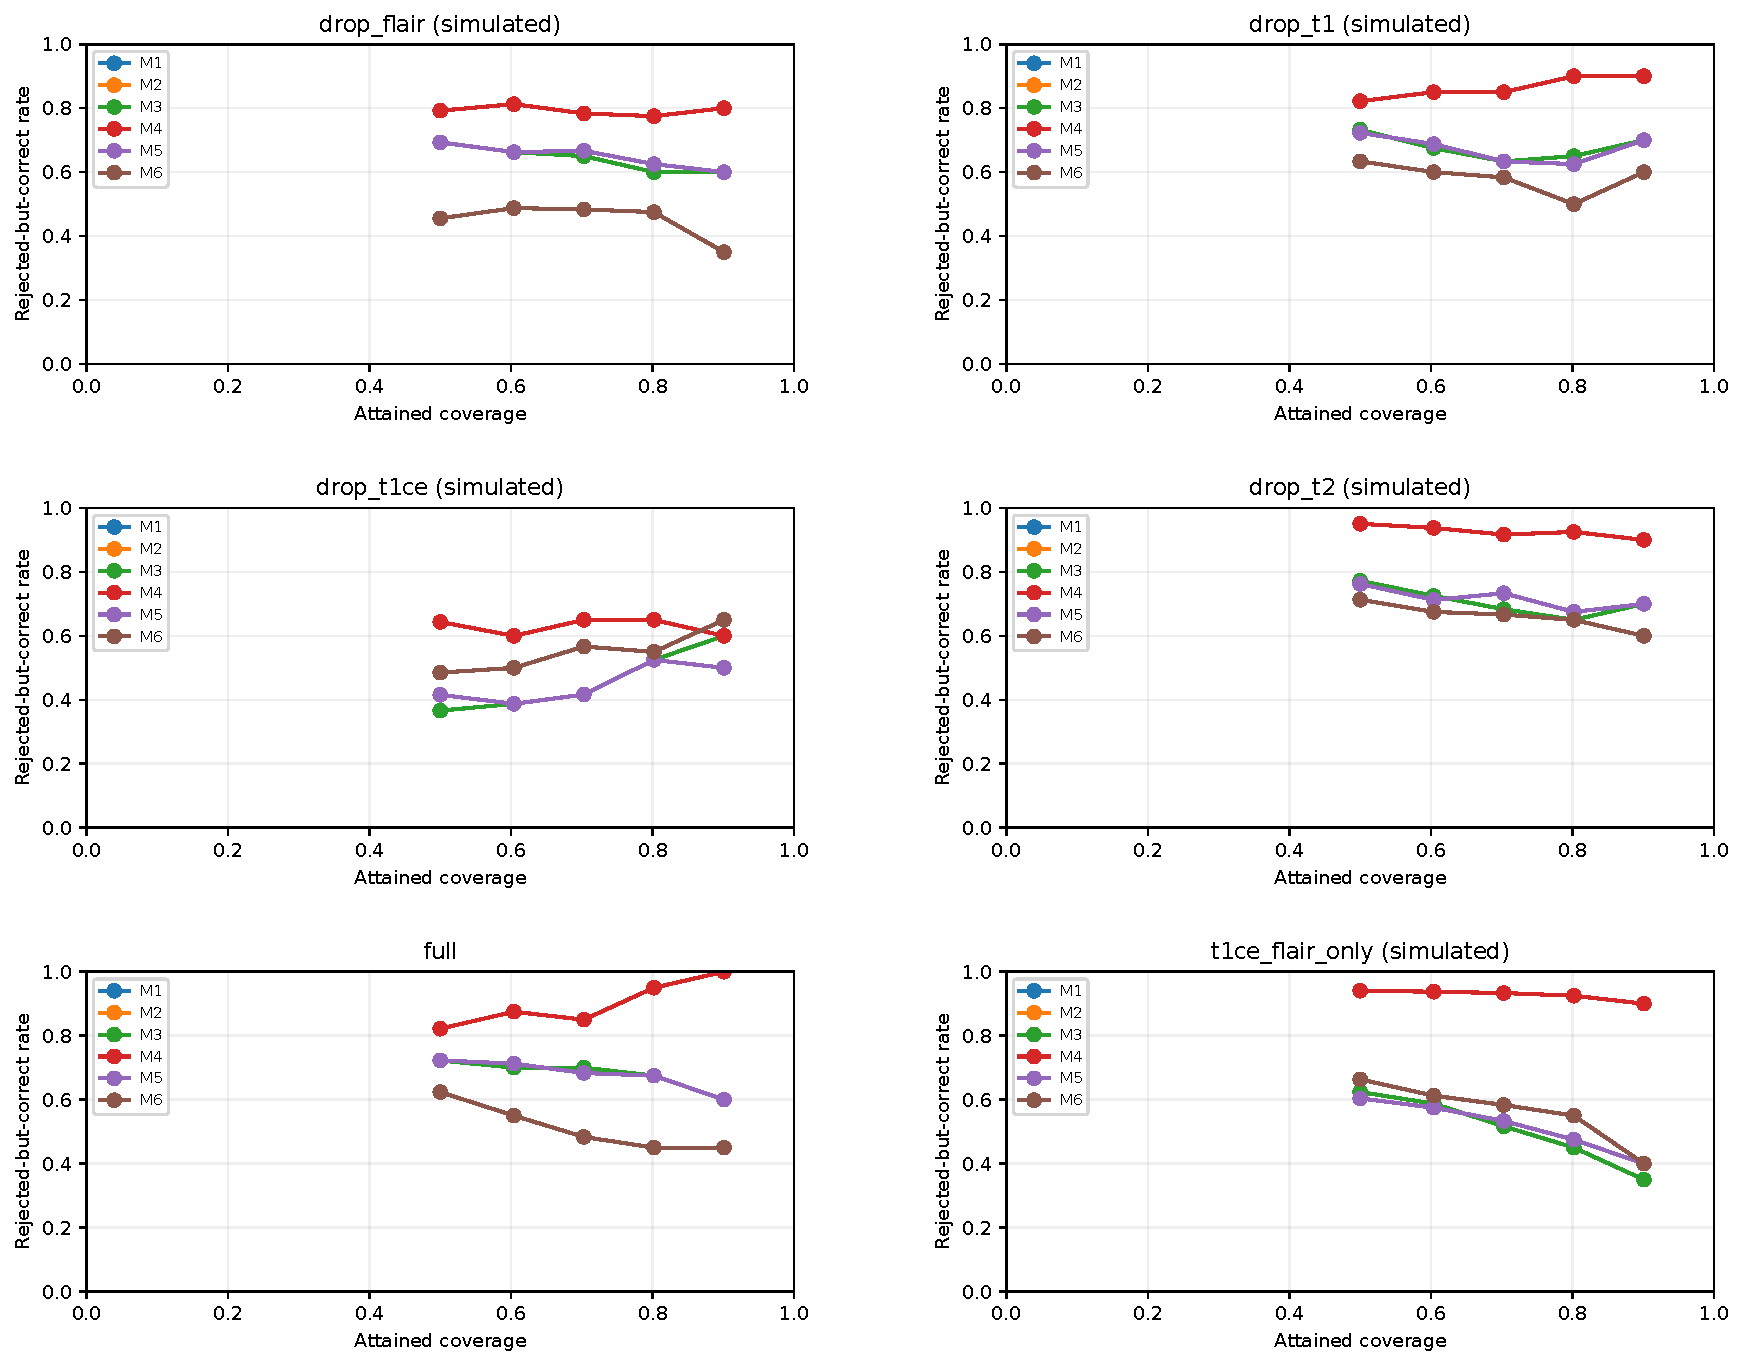
\includegraphics[width=0.78\textwidth]{figures/journal_fig_abst_ucsf.pdf}
\caption{Rejected-but-correct rate against attained coverage on UCSF-PDGM, by condition and mechanism. No intervals are stored for this rate. Missing-sequence conditions are simulated.}
\label{fig:abst}
\end{figure*}

\subsection{Does Conformal Coverage Hold? (RQ2, C4)}
Table~\ref{tab:cov} gives set coverage on complete input, and Table~\ref{tab:sets} gives the composition of the prediction sets. The carried-over quantiles were \numIntQuantAlphafive{}, \numIntQuantAlphaten{}, and \numIntQuantAlphatwenty{} for $\alpha=0.05$, 0.1, and 0.2, with calibration-split coverage \numIntCalCovAlphafive{}, \numIntCalCovAlphaten{}, and \numIntCalCovAlphatwenty{}. At $\alpha=0.05$ the external coverage was \numExtCovAlphafive{} against a nominal 0.95, inside the $\pm0.07$ band. At $\alpha=0.1$ it was \numExtCovAlphaten{} against 0.90, and at $\alpha=0.2$ it was \numExtCovAlphatwenty{} against 0.80, with \numExtEmptyAlphatwenty{} of the $\numNExt$ prediction sets empty. At $\alpha=0.1$ and 0.2 the external deviation intervals were wider than the band in every condition; at $\alpha=0.05$ five of six conditions passed and T1ce removal did not (half-width \numExtHalfAlphafiveDropTonece). Internally, all but one of the condition--$\alpha$ cells exceeded the band (Table~\ref{tab:confint}). C4 is therefore refuted: at these sample sizes the intervals cannot separate preserved from degraded coverage. This is a statement about the precision of the measurement, not a finding that coverage holds or fails.

The internal test split, which is exchangeable with the calibration split by construction, shows deviations of similar size. At $\alpha=0.2$ the calibration coverage was \numIntCalCovAlphatwenty{} but the internal test coverage was \numIntCovAlphatwenty{} (nominal 0.80), a shortfall of the same order as the external one (\numExtCovAlphatwenty{}). Much of the apparent deviation at this sample size is therefore sampling noise from a 124-patient calibration set and cannot be attributed to shift.

\begin{table}[t]
\centering
\caption{Conformal Set Coverage on Complete Input, Quantiles From the UTSW Calibration Split. Half Is the Half-Width of the Coverage-Deviation Interval}
\label{tab:cov}
\footnotesize
\begin{tabular}{lccccc}
\toprule
 & & \multicolumn{2}{c}{UTSW test} & \multicolumn{2}{c}{UCSF-PDGM} \\
$\alpha$ & Nominal & Cov. & Half & Cov. & Half \\
\midrule
0.05 & 0.95 & \numIntCovAlphafive & \numIntHalfAlphafive & \numExtCovAlphafive & \numExtHalfAlphafive \\
0.10 & 0.90 & \numIntCovAlphaten & \numIntHalfAlphaten & \numExtCovAlphaten & \numExtHalfAlphaten \\
0.20 & 0.80 & \numIntCovAlphatwenty & \numIntHalfAlphatwenty & \numExtCovAlphatwenty & \numExtHalfAlphatwenty \\
\bottomrule
\end{tabular}
\end{table}

\begin{table}[t]
\centering
\caption{Composition of Conformal Prediction Sets on Complete Input: Abstention Rate (Empty or Two-Label Sets), Counts of Empty and Two-Label Sets, and Accuracy Among Singleton Sets}
\label{tab:sets}
\footnotesize
\setlength{\tabcolsep}{4pt}
\begin{tabular}{llcccc}
\toprule
Cohort & $\alpha$ & Abstain & Empty & Two-label & Singleton acc. \\
\midrule
UTSW test & 0.05 & \numIntAbstAlphafive & \numIntEmptyAlphafive & \numIntFullAlphafive & \numIntSingleTrueAlphafive \\
 & 0.10 & \numIntAbstAlphaten & \numIntEmptyAlphaten & \numIntFullAlphaten & \numIntSingleTrueAlphaten \\
 & 0.20 & \numIntAbstAlphatwenty & \numIntEmptyAlphatwenty & \numIntFullAlphatwenty & \numIntSingleTrueAlphatwenty \\
UCSF-PDGM & 0.05 & \numExtAbstAlphafive & \numExtEmptyAlphafive & \numExtFullAlphafive & \numExtSingleTrueAlphafive \\
 & 0.10 & \numExtAbstAlphaten & \numExtEmptyAlphaten & \numExtFullAlphaten & \numExtSingleTrueAlphaten \\
 & 0.20 & \numExtAbstAlphatwenty & \numExtEmptyAlphatwenty & \numExtFullAlphatwenty & \numExtSingleTrueAlphatwenty \\
\bottomrule
\end{tabular}
\end{table}

The set composition explains the pattern of coverage across $\alpha$. At $\alpha=0.05$ and 0.1 the quantile is large enough that no set is empty, so every miscovered patient is a confident singleton error, and the two-label sets act as abstentions; the external abstention rate at $\alpha=0.05$ was \numExtAbstAlphafive{} against \numIntAbstAlphafive{} internally. At $\alpha=0.2$ the quantile falls below 0.5, no set holds both labels, and each patient whose larger class probability lies below $1-\hat q_{0.2}$ receives an empty set. Empty sets are miscoverages by definition, so they account for much of the shortfall at $\alpha=0.2$. Accuracy among singleton sets stayed high on both cohorts.

Figs.~\ref{fig:covint} and~\ref{fig:cov} show coverage for every condition, for the carried-over and the refit quantiles. Most conditions sit near the diagonal at $\alpha=0.05$ and drift below it at $\alpha=0.2$. With T1ce removed the carried-over coverage falls far below nominal and is labeled degraded at $\alpha=0.1$ and 0.2 internally and at $\alpha=0.2$ externally (Tables~\ref{tab:confint} and~\ref{tab:confext}), while the refit variant, which recomputes the quantile on the calibration split with T1ce removed, stays at or above nominal. The deviation in that condition is therefore a shift in the score distribution caused by the missing sequence, and it is corrected when the calibration data have the same missing pattern as the test data. The refit variant is a diagnostic, not the frozen method.

\begin{figure*}[t]
\centering
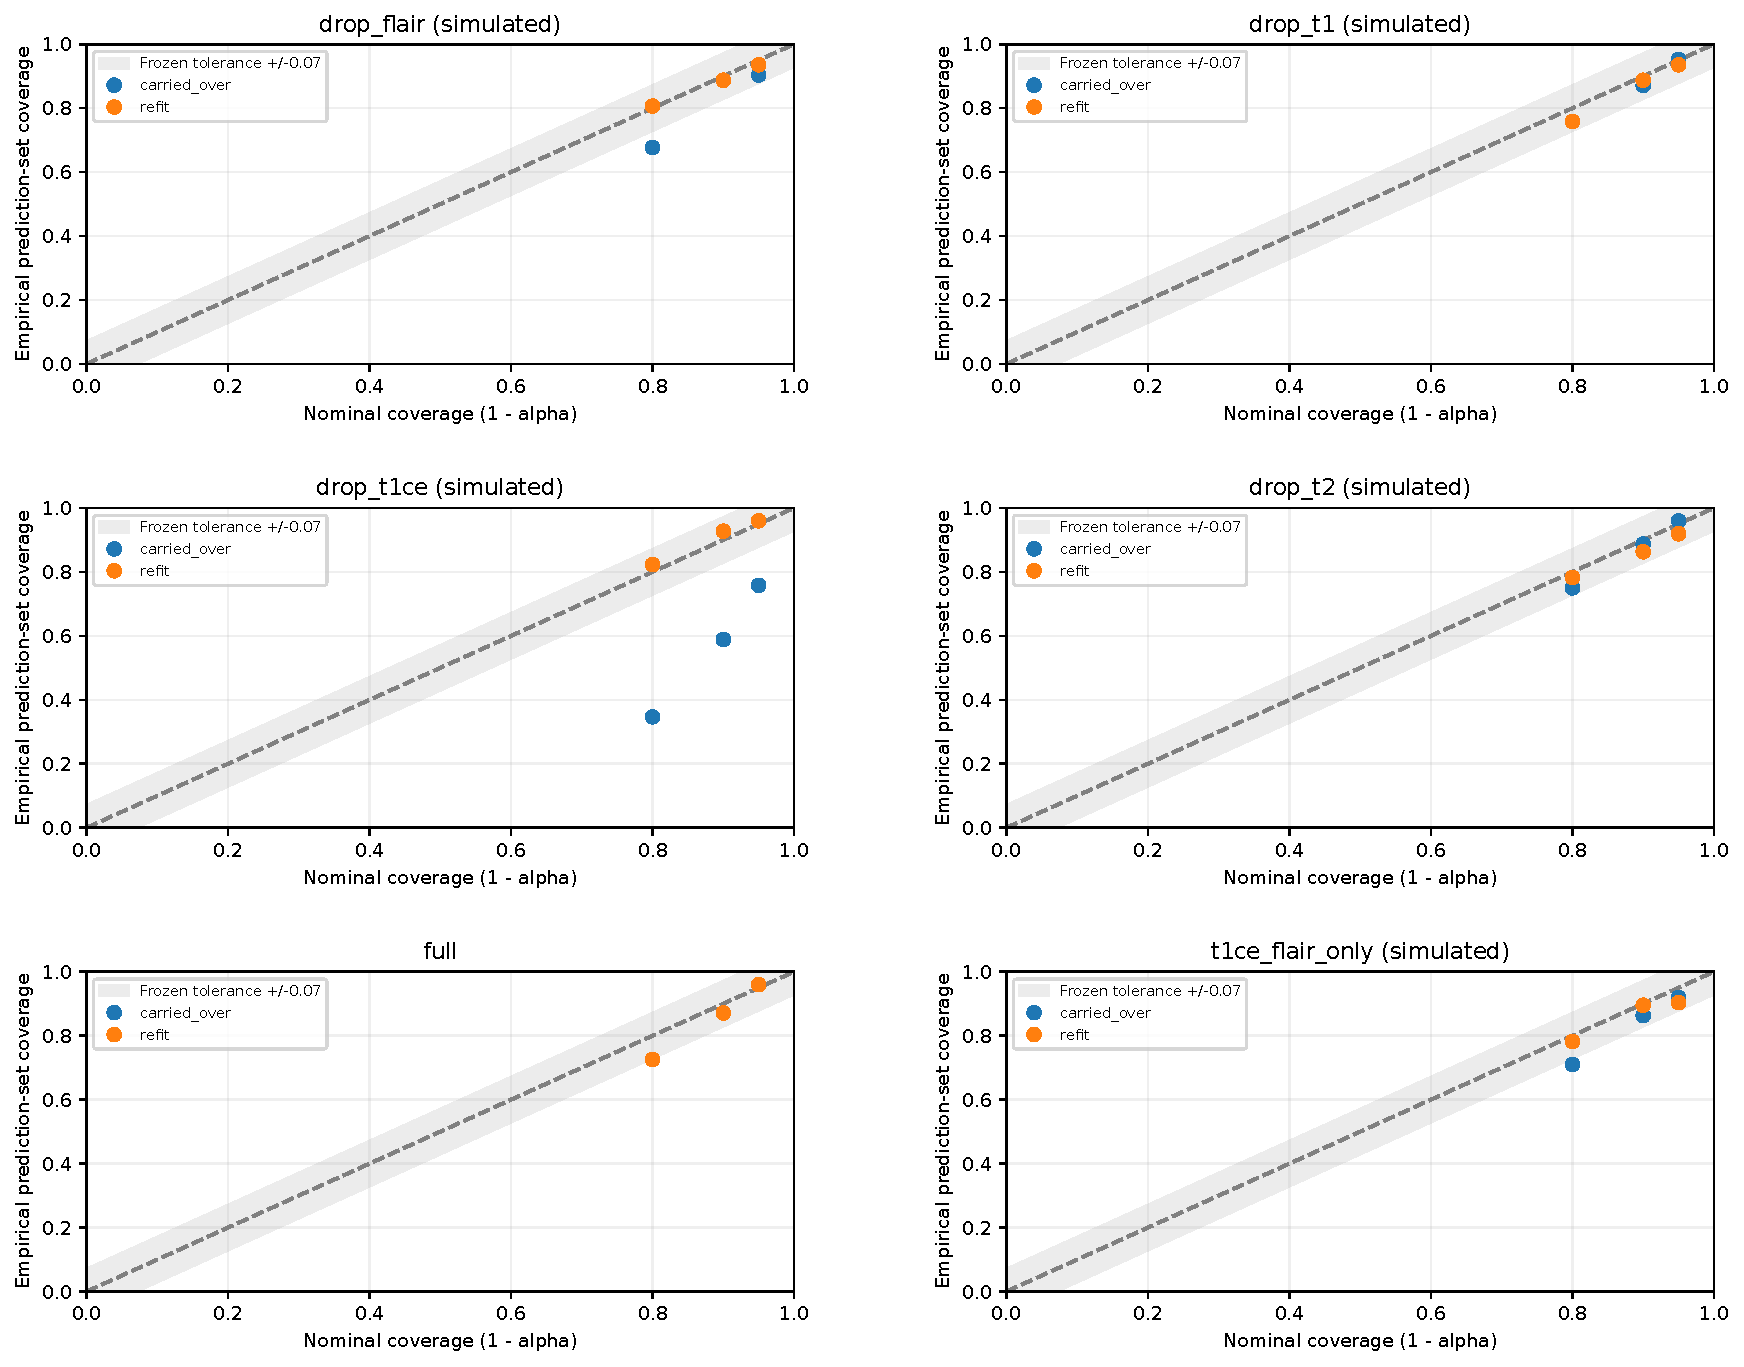
\includegraphics[width=0.78\textwidth]{figures/journal_fig_cov_utsw.pdf}
\caption{Nominal against empirical conformal set coverage on the UTSW internal test split by condition, carried-over and refit quantiles. The shaded band is the frozen $\pm0.07$ tolerance, not an interval. Missing-sequence conditions are simulated.}
\label{fig:covint}
\end{figure*}

\begin{figure*}[t]
\centering
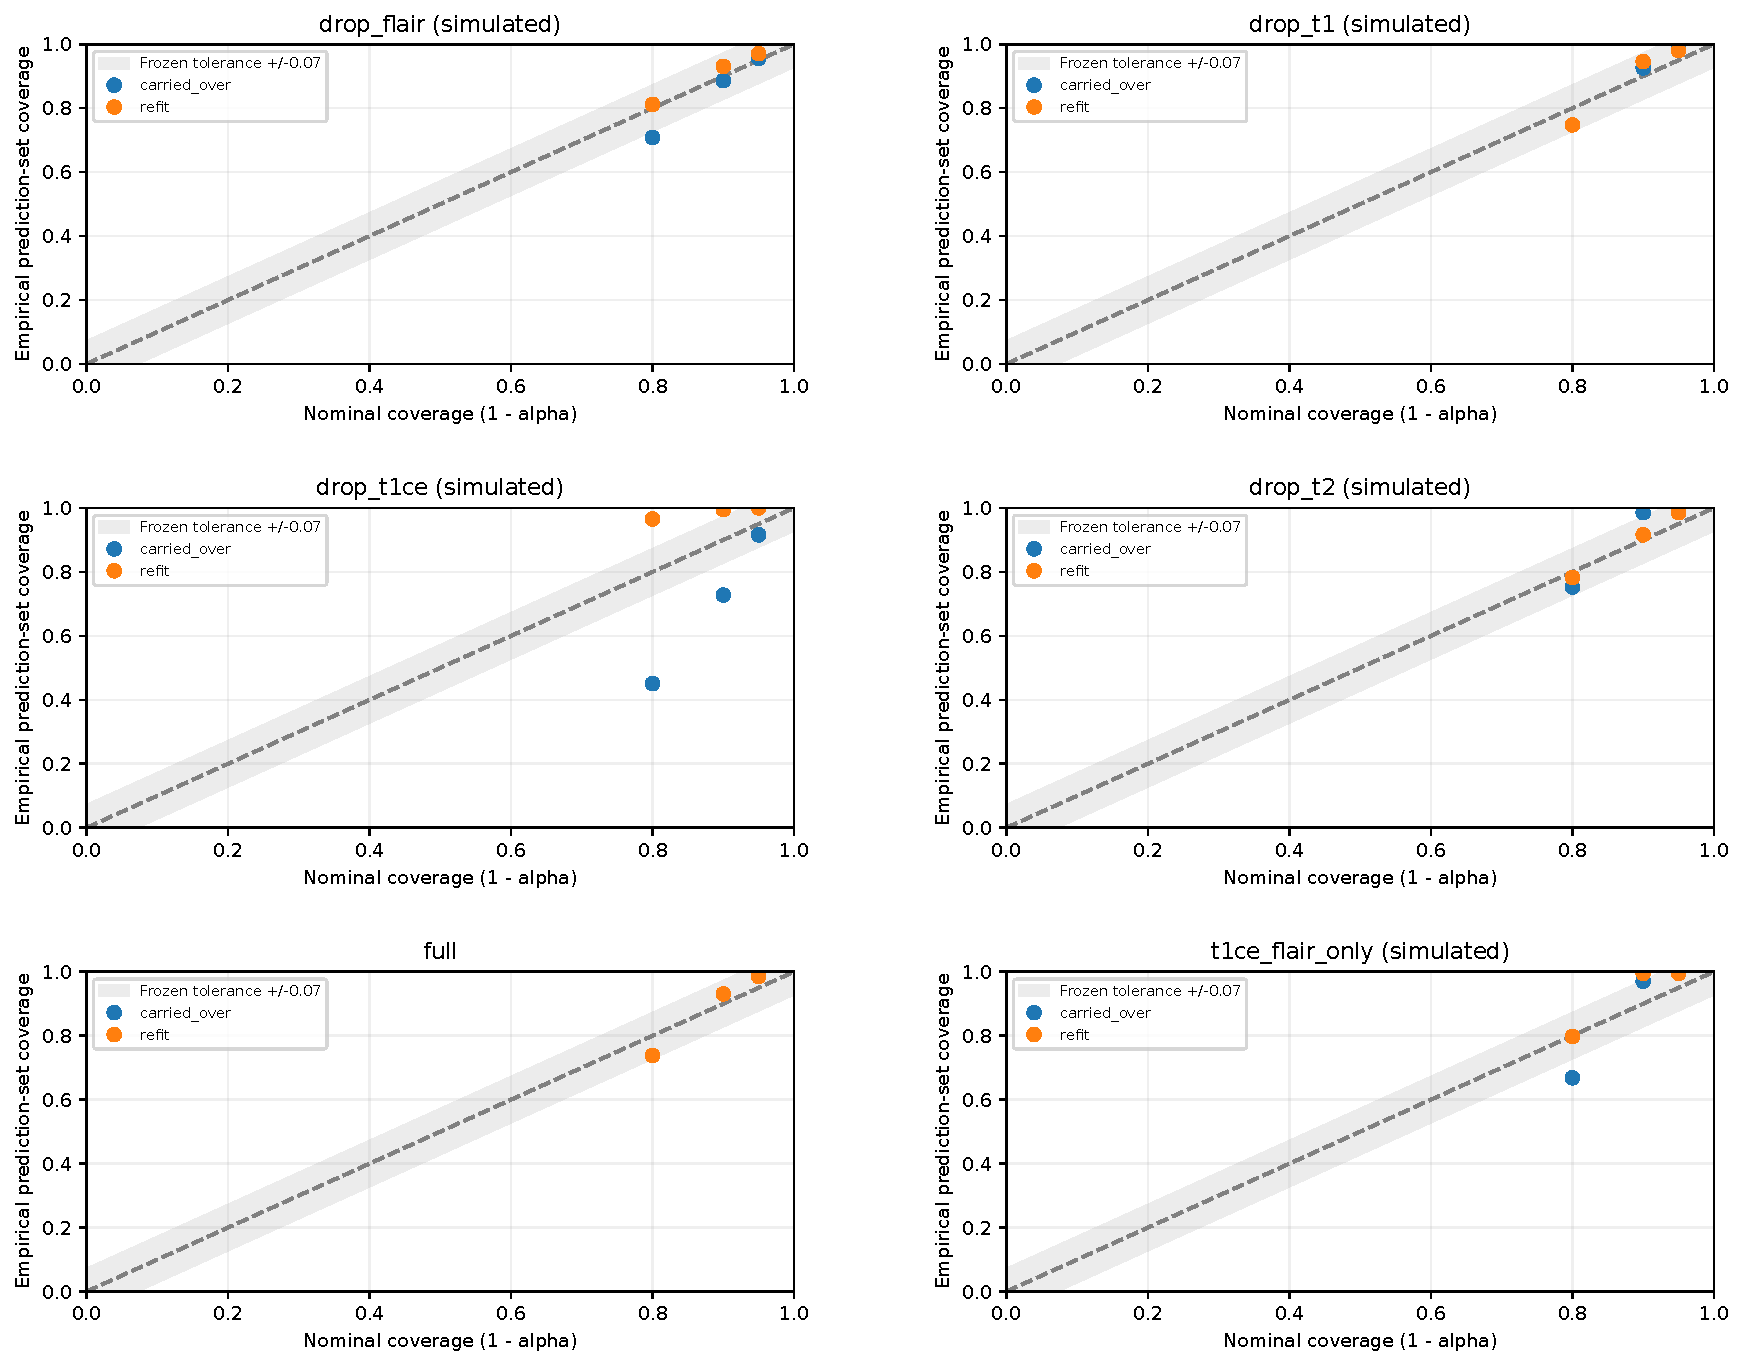
\includegraphics[width=0.78\textwidth]{figures/journal_fig_cov_ucsf.pdf}
\caption{Nominal against empirical conformal set coverage on UCSF-PDGM by condition, carried-over and refit quantiles. The shaded band is the frozen $\pm0.07$ tolerance, not an interval. Missing-sequence conditions are simulated.}
\label{fig:cov}
\end{figure*}

\subsection{Internal Against External AURC}
The single unpaired contrast of external against internal AURC on complete input (block C) was \numExtCOneDiff{} (95\% interval \numExtCOneLo{} to \numExtCOneHi{}; adjusted $p=\numFamXCOneAdj$). The external AURC was not detectably different from the internal one. Together with the calibration result, this shows no measurable penalty from the institutional shift on complete input in this pair of cohorts.

\subsection{Ablations (Family Block E)}
R7 and R8 did not differ from R2 on UTSW (adjusted $p$ of \numFamUEOneAdj, \numFamUETwoAdj, \numFamUEThreeAdj, and \numFamUEFourAdj{} for the four contrasts). On UCSF-PDGM R7 had a worse AURC than R2 (difference \numExtETwoDiff, adjusted $p=\numFamXETwoAdj$) and a nonsignificant AUROC difference (\numExtEOneDiff, adjusted $p=\numFamXEOneAdj$); R8 was not distinguishable from R2 (AUROC difference \numExtEThreeDiff, adjusted $p=\numFamXEThreeAdj$; AURC difference \numExtEFourDiff, adjusted $p=\numFamXEFourAdj$). The evidence for tumor-aware pooling is one AURC contrast on one cohort.

\subsection{Auxiliary Segmentation}
Table~\ref{tab:seg} gives segmentation quality on the internal test split. The primary model reached a mean Dice of \numDiceRTwo{}, with median 95th-percentile Hausdorff distances (HD95) of \numHdEnhRTwo{}, \numHdCoreRTwo{}, and \numHdOedRTwo{}\,mm (enhancing tumor, core, and edema) over evaluable patients. The two-stage model, whose first stage is trained on segmentation alone, segmented much better (mean Dice \numDiceREight{}) without a corresponding gain in IDH discrimination. Segmentation was an auxiliary task and is not part of the claims.

\begin{table}[t]
\centering
\caption{Auxiliary Segmentation on the UTSW Internal Test Split: Dice and Median HD95 (mm, Evaluable Patients)}
\label{tab:seg}
\footnotesize
\resizebox{\columnwidth}{!}{\begin{tabular}{lrrrrrrr}
\toprule
Run & Dice & Enh. & Core & Edema & HD95 enh. & HD95 core & HD95 ed. \\
\midrule
R2 (primary) & 0.473 & 0.431 & 0.390 & 0.597 & 7.5 & 9.2 & 8.5 \\
R7 (global pooling) & 0.485 & 0.481 & 0.409 & 0.566 & 6.0 & 11.0 & 9.8 \\
R8 (two-stage) & 0.741 & 0.799 & 0.605 & 0.819 & 2.0 & 6.2 & 3.5 \\
\bottomrule
\end{tabular}
}
\end{table}

\subsection{1p/19q Probe (RQ4, Exploratory)}
A frozen-encoder probe (L2-regularized logistic regression on 256 features, fitted on the \numProbeTrainN{} UTSW training patients with a label, \numProbeTrainCodel{} codeleted, and scored on the \numProbeN{} internal-test patients with a label, \numProbeCodel{} codeleted) reached an AUROC of \numProbeAuroc{} (95\% bootstrap interval \numProbeAurocLo{} to \numProbeAurocHi{}; Table~\ref{tab:probe}). All codeleted patients in this test set are IDH-mutant, so the all-patient AUROC partly re-reads IDH status; the IDH probability alone reached \numProbeIdhAuroc{}. Inside the \numProbeMutN{} IDH-mutant patients the probe ranked codeleted patients above the rest (AUROC \numProbeMutAuroc{}, interval \numProbeMutAurocLo{} to \numProbeMutAurocHi{}) where the IDH probability did not (\numProbeMutIdhAuroc{}); the probe interval includes 0.5, so this is descriptive only. No external 1p/19q evaluation was run, and the selective-prediction analysis was not extended to 1p/19q.

\begin{table}[t]
\centering
\caption{1p/19q Frozen-Encoder Probe on the UTSW Internal Test Split (Exploratory)}
\label{tab:probe}
\footnotesize
\resizebox{\columnwidth}{!}{\begin{tabular}{lrrccc}
\toprule
Subset & $n$ & Codel. & Probe AUROC [95\%] & AUPRC & IDH-prob. AUROC \\
\midrule
All labeled patients & 66 & 14 & 0.787 [0.627, 0.919] & 0.587 & 0.714 \\
IDH-mutant only & 28 & 14 & 0.673 [0.441, 0.870] & 0.763 & 0.337 \\
\bottomrule
\end{tabular}
}
\end{table}

\subsection{Multiplicity and the Confirmatory Family}
Of the $\numFamilySize$ family tests, $\numFamilyRejected$ are rejected at $q=0.05$ (Table~\ref{tab:family}). They are the T1ce-removal AURC increase on UTSW; and on UCSF-PDGM, the M5-against-M4 and MC-dropout-against-M4 contrasts, the T1ce-removal and FLAIR-removal AURC increases, the raw-against-scaled Brier contrast, and the R7-against-R2 AURC contrast. No UTSW block A, D, or E member and no UCSF block C member was rejected. Several rejected members sit on the permutation floor ($p=2/2001$), so their adjusted $p$ is the floor times the family size over rank, and it bounds the evidence instead of measuring it.

\subsection{Claim Adjudication}
Table~\ref{tab:claims} lists every claim under the frozen rules. Refuted claims are reported as refuted: C2, C4 (on both cohorts), and C6 (internally). C1 is supported internally, C3 is supported on complete input externally (worst over the five missing-sequence conditions: inconclusive), and C5 is supported externally and inconclusive internally.

\begin{table}[t]
\centering
\caption{Pre-Registered Claims and Their Frozen-Rule Status}
\label{tab:claims}
\footnotesize
\begin{tabular}{lll}
\toprule
Claim & UTSW (internal) & UCSF-PDGM (external) \\
\midrule
C1 & \numStatusCOneInt & --- \\
C2 & \numStatusCTwoInt & --- \\
C3 & --- & \numStatusCThreeExt{} (full); worst \numStatusCThreeWorst \\
C4 & \numStatusCFourInt & \numStatusCFourExt \\
C5 & \numStatusCFiveInt & \numStatusCFiveExt \\
C6 & \numStatusCSixInt & \numStatusCSixExt \\
\bottomrule
\end{tabular}
\end{table}

\subsection{Independent Verification}
\label{sec:verification}
A second software agent recomputed the external numbers from the written contracts and the frozen prediction files, with its results file written before it opened any author result. Most compared quantities agreed. The differences were traced to four causes: a tie-handling ambiguity in the oracle AURC definition (we kept the strictly ordered reading, the lowest value any ordering reaches); the Monte Carlo seed layout for permutation tests and the two-stage bootstrap (the agent reproduced the coverage intervals and the unpaired-comparison $p$-value of the author exactly once the seed schedule was given); a $4\times10^{-9}$ difference in the fitted temperature from an independent solver, inside the stated tolerance; and a labeling error in the agent's own summary of claim C3. No reported value, claim status, or rejection changed. The contracts did not fix the external seed schedule; it is documented in the analysis file and should be stated in the contracts.

\section{Discussion}
\label{sec:discussion}

\subsection{Answers to the Research Questions}
\textbf{RQ1.} On complete input, abstaining lowers selective risk below the always-predict risk at every coverage level from 0.5 to 0.9, on both cohorts. The curves are monotone on the external cohort, so we did not observe the non-monotone referral failure reported for other imaging domains \cite{srivastava2023}. The advantage does not hold for every missing sequence. With T1ce removed, the internal advantage is lost (C2 refuted), and the external advantage is only inconclusive. Conformal prediction adds no ranking advantage over temperature-scaled confidence.

\textbf{RQ2.} Conformal coverage could not be characterized within the pre-registered $\pm0.07$ tolerance at this sample size (C4 refuted on both cohorts). The point estimates are above nominal at $\alpha=0.05$ and 0.1 and below it at $\alpha=0.2$, with many empty sets, so there is no simple pattern of degradation. The internal test split shows deviations of similar size, so much of the observed external deviation is consistent with small-sample noise in the calibration quantile. The one condition with a clear shift effect is T1ce removal, and recalibrating on data with the same missing pattern removes it.

\textbf{RQ3.} We observed no degradation of calibration from the internal to the external cohort. This is a descriptive comparison with overlapping intervals, from one architecture and two cohorts.

\textbf{RQ4.} The exploratory probe suggests some 1p/19q signal inside IDH-mutant patients, but the interval includes 0.5. No selective-prediction conclusion for 1p/19q is drawn.

\subsection{Why Does Removing T1ce Matter?}
T1ce carries the contrast-enhancement signal on which tumor-aware features rely. Removing it lowered discrimination and, more importantly for abstention, left the model no better at knowing when it was wrong: internally the least confident cases were no more likely to be errors than random cases (C6 refuted), and the confidence ranking barely improved on the always-predict risk. The reliability diagram in the same condition shows why: predictions above one half are often wrong, so confidence no longer tracks correctness. The model trained without modality dropout (M6) degraded much more sharply when T1ce was removed, which is the expected benefit of modality dropout \cite{neverova2016} and was not part of any claim. A deployed system should treat a missing T1ce as a reason to withhold the prediction or to request the missing sequence, not as a condition to handle with a lowered threshold.

\subsection{Why Does Ensemble Disagreement Rank Errors Poorly on Complete Input?}
The ensemble-variance score ranks only by disagreement between members, which ignores how confident the members are on average. On complete input all members agree on most easy cases, and a patient whom every member confidently misclassifies has low variance and is accepted early. The rejected-but-correct rate of M4 was correspondingly high. The confidence score uses the average probability and ranked better externally (UCSF A2 and A3 rejected). With T1ce removed internally, members disagree more where the input is uninformative, and disagreement became a better error signal (M4 AURC below M2). Benchmarks of uncertainty under shift found ensembles among the best calibrated methods \cite{ovadia2019}; our result concerns ranking by variance alone, not the calibration of the ensemble mean. We did not pre-specify that contrast, so it is a hypothesis, not a finding.

\subsection{Sample Size and the Coverage Guarantee}
The coverage result is first a statement about measurement precision. With 124 calibration patients, the quantile that defines a 90\% set is estimated from a tail of about a dozen scores, and with 124 or 202 test patients the empirical coverage has a binomial standard error of 0.02 to 0.03 before calibration variability is added. The two-stage bootstrap adds that variability, which is why the half-widths in Table~\ref{tab:cov} are larger than a binomial interval would suggest. A 0.07 band therefore cannot be verified at $\alpha=0.1$ or 0.2, and no feasible split of a 616-patient cohort reaches it. Our finding does not show that the conformal guarantee breaks under shift; it shows that, at this scale, a coverage study cannot say.

\subsection{Calibrating on the Missing Pattern}
The refit diagnostic suggests a practical remedy for the one condition that clearly broke coverage. Under T1ce removal the carried-over quantile, fitted on complete input, was too small for the shifted score distribution, and coverage fell; a quantile computed on calibration patients with T1ce removed restored it. Because the missing pattern is known at inference, a system can hold one calibration quantile per pattern, which is the Mondrian idea of conditioning calibration on an observed category \cite{vovk2005}. That remedy costs nothing at training time but needs calibration data for each pattern, and it does not repair the ranking: under T1ce removal more patients receive two-label sets (Table~\ref{tab:confint}), because the model is less informative. It is a hypothesis for future work, not a tested method here.

\subsection{Calibration Did Not Degrade, and Temperature Scaling Did Not Help}
A recent comparison of IDH models with physicians found the best physicians better calibrated than the models on external data \cite{takahashi2026}. We did not see degradation: the external ECE and Brier score were similar to or lower than the internal ones. With two cohorts, one architecture, and a filtered external cohort, we do not claim this generalizes. Temperature scaling did not lower ECE on either cohort. The fitted temperature was near one, the calibration split was also used for early stopping, and the network was trained with a class-weighted loss and modality dropout, any of which may already have produced reasonably calibrated outputs. With 124 calibration patients and ten bins, the ECE itself is a noisy estimate, so small differences between raw and scaled ECE should not be read as effects.

\subsection{Clinical Implications}
For a user of such a system, the results support three practical points, each limited to the settings we tested. First, abstaining on the least confident half of cases removed most of the errors on complete input, so a flag-for-review workflow is plausible for complete studies. Second, a missing contrast-enhanced sequence should itself trigger abstention or a request for the sequence. Third, a conformal set rule needs a calibration set large enough, and ideally drawn from the deployment site and the deployed protocol, before its nominal coverage can be trusted. None of these points is validated prospectively, and we make no claim about clinical benefit.

\subsection{Relation to Prior Work}
Our complete-input result is consistent with prior conformal work that reports useful coverage on complete sequences \cite{elyassirad2026}, and with referral studies in which rejecting uncertain cases improved accuracy on the rest \cite{leibig2017,olsson2022}. We add that the advantage depends on which sequence is missing, that the coverage deviation cannot be bounded within a 0.07 band at these sample sizes, and that the conformal ranking is equivalent to temperature-scaled confidence. The comparison with imputation-based missing-sequence methods \cite{liang2026risen} is indirect, because those methods always predict and report discrimination; testing whether imputation followed by abstention beats zeroing followed by abstention is a natural follow-up.

\subsection{Strengths}
The claims and decision rules were fixed before any external result was seen. The external evaluation ran once under a signed manifest and a harness that checks hashes and repository state. Negative results are reported plainly and were not re-run. Every number in the text is generated from frozen files, the figures and tables regenerate byte for byte, and an independent recomputation of the external numbers found no discrepancy that changed a reported value.

\section{Limitations}
\label{sec:limits}
\begin{itemize}[leftmargin=1.2em]
\item \textbf{Simulated missingness.} All three cohorts are curated four-sequence studies, so missing sequences were simulated by zeroing a channel. That reproduces the information loss but not the real selection mechanism (motion, intolerance, truncated protocols, scanner failure), which may correlate with image quality or disease severity. Every missing-sequence table and caption says ``simulated,'' and the claim wording was not softened after the fact. Naturally missing sequences were excluded to keep the patient set identical across conditions.
\item \textbf{Sample size.} The internal-test split has $\numNIntPos$ mutant patients and the external cohort $\numNExtPos$, so intervals are wide. Coverage-deviation intervals cannot meet the 0.07 band at $\alpha=0.1$ or 0.2.
\item \textbf{One development institution}, and one external cohort after excluding BraTS-overlapping patients, which changes the label mix. EGD is deferred.
\item \textbf{Labels.} UTSW IDH labels mix immunohistochemistry (66\%) and sequencing (34\%), with a differential false-negative risk for non-R132H variants. Label harmonization was done by one reviewer. The UCSF-PDGM assay was not independently reconfirmed.
\item \textbf{Calibration split reuse.} The calibration split served early stopping as well as temperature scaling and conformal quantiles, which may make calibration slightly optimistic.
\item \textbf{1p/19q} was examined only internally with a frozen-encoder probe, exploratory, with no inferential claim and no selective-prediction analysis.
\item \textbf{Single architecture.} We did not compare backbones, by design, so conclusions are about this network family.
\item \textbf{Review depth.} The team was one researcher. Independent checks (phase reviews and the recomputation of the external numbers) were done by a second software agent working from written contracts, not by a second person. Every reported number matched except for differences traced to the causes in Section~\ref{sec:verification}.
\item \textbf{Protocol deviation.} The first external manifest omitted R7 and R8. A second signed manifest and run corrected it before any external metric was examined, with no change of method.
\item \textbf{Oracle AURC reading.} The contract sentence defining the oracle AURC is ambiguous about ties; we kept the strictly ordered reading and flag it here. No claim depends on it.
\end{itemize}

\section{Future Work}
\label{sec:future}
The external evaluation on EGD is planned as a second, separately frozen evaluation that does not join the primary result. A larger calibration set from the deployment institution would test whether the coverage guarantee can be verified within a tight band. Per-pattern calibration, suggested by the refit diagnostic, should be tested as a pre-specified method on new data. Real incomplete protocols, where available, would test whether simulated and natural missingness behave alike. An imputation-then-abstain comparison would connect this work to imputation-based methods. A prospective reader study would be needed to measure whether the abstain-and-review workflow changes clinical decisions.

\section{Conclusion}
Abstention helped where the input was complete and stopped helping when T1ce was missing. Conformal coverage could not be characterized within the pre-registered tolerance at these sample sizes, the one clear coverage failure came from the missing contrast-enhanced sequence, and calibration did not degrade from the internal to the external cohort. Four of six claims were not supported in at least one cohort, and we report them as such. The code, the frozen predictions, and the generation scripts allow every number and figure to be rebuilt.

\clearpage
\onecolumn
\appendices

\section{Full Per-Condition Tables}
\label{app:tables}
This appendix gives the full per-condition results behind the summaries in Section~\ref{sec:results}, all generated from the frozen result files: $D(\phi)$ for every condition and cohort (Tables~\ref{tab:deltaint} and~\ref{tab:deltaext}), the monotonicity differences (Table~\ref{tab:mono}), the abstention enrichment tests (Tables~\ref{tab:enrichint} and~\ref{tab:enrichext}), conformal set coverage by condition and $\alpha$ (Tables~\ref{tab:confint} and~\ref{tab:confext}), and the full $\numFamilySize$-test family (Table~\ref{tab:family}). Missing-sequence conditions are simulated throughout.

\begin{table}[!ht]
\centering
\caption{$D(\phi)$ Point Estimate and (Upper 95\% Limit) by Condition on the UTSW Internal Test Split. A Positive Value Means Worse Than Always Predicting}
\label{tab:deltaint}
\footnotesize
\begin{tabular}{lccccc}
\toprule
Condition & 0.5 & 0.6 & 0.7 & 0.8 & 0.9 \\
\midrule
Full & -0.169 (-0.097) & -0.124 (-0.070) & -0.103 (-0.044) & -0.058 (-0.020) & -0.048 (-0.009) \\
$-$T1 (sim.) & -0.129 (-0.058) & -0.084 (-0.020) & -0.051 (-0.004) & -0.027 (+0.012) & -0.017 (+0.016) \\
$-$T1ce (sim.) & +0.016 (+0.118) & +0.054 (+0.126) & +0.065 (+0.136) & +0.048 (+0.095) & +0.012 (+0.043) \\
$-$T2 (sim.) & -0.105 (-0.048) & -0.105 (-0.048) & -0.094 (-0.038) & -0.055 (-0.013) & -0.052 (-0.010) \\
$-$FLAIR (sim.) & -0.145 (-0.065) & -0.092 (-0.023) & -0.076 (-0.018) & -0.046 (-0.012) & -0.038 (-0.001) \\
T1ce+FLAIR (sim.) & -0.056 (+0.014) & -0.058 (+0.006) & -0.045 (-0.002) & -0.038 (+0.008) & -0.021 (+0.013) \\
\bottomrule
\end{tabular}

\end{table}

\begin{table}[!ht]
\centering
\caption{$D(\phi)$ Point Estimate and (Upper 95\% Limit) by Condition on UCSF-PDGM}
\label{tab:deltaext}
\footnotesize
\begin{tabular}{lccccc}
\toprule
Condition & 0.5 & 0.6 & 0.7 & 0.8 & 0.9 \\
\midrule
Full & -0.124 (-0.066) & -0.088 (-0.043) & -0.069 (-0.036) & -0.042 (-0.015) & -0.027 (-0.006) \\
$-$T1 (sim.) & -0.114 (-0.064) & -0.098 (-0.054) & -0.086 (-0.041) & -0.052 (-0.020) & -0.015 (+0.004) \\
$-$T1ce (sim.) & -0.134 (-0.073) & -0.106 (-0.048) & -0.056 (-0.002) & -0.006 (+0.030) & -0.005 (+0.019) \\
$-$T2 (sim.) & -0.109 (-0.064) & -0.104 (-0.058) & -0.058 (-0.026) & -0.048 (-0.017) & -0.019 (+0.001) \\
$-$FLAIR (sim.) & -0.104 (-0.045) & -0.088 (-0.044) & -0.055 (-0.019) & -0.042 (-0.013) & -0.022 (-0.003) \\
T1ce+FLAIR (sim.) & -0.188 (-0.120) & -0.142 (-0.093) & -0.109 (-0.067) & -0.078 (-0.044) & -0.043 (-0.021) \\
\bottomrule
\end{tabular}

\end{table}

\begin{table}[!ht]
\centering
\caption{Adjacent-Coverage Risk Differences (Lower Minus Higher Coverage), the Largest Lower 95\% Limit, and the Number of Violating Adjacent Cutoff Pairs, by Condition. Top: UTSW Internal; Bottom: UCSF-PDGM}
\label{tab:mono}
\footnotesize
\begin{tabular}{lcccccc}
\toprule
Condition & 0.5--0.6 & 0.6--0.7 & 0.7--0.8 & 0.8--0.9 & Max lower & Viol. \\
\midrule
Full & -0.010 & -0.045 & -0.022 & -0.045 & -0.060 & 253 \\
$-$T1 (sim.) & -0.011 & -0.024 & -0.033 & -0.045 & -0.052 & 422 \\
$-$T1ce (sim.) & +0.035 & +0.018 & -0.011 & -0.038 & -0.001 & 1467 \\
$-$T2 (sim.) & -0.004 & -0.038 & -0.012 & +0.001 & -0.049 & 361 \\
$-$FLAIR (sim.) & -0.008 & -0.031 & -0.016 & -0.053 & -0.061 & 604 \\
T1ce+FLAIR (sim.) & -0.016 & -0.008 & -0.012 & +0.001 & -0.047 & 416 \\
\bottomrule
\end{tabular}
 \\[6pt]
\begin{tabular}{lcccccc}
\toprule
Condition & 0.5--0.6 & 0.6--0.7 & 0.7--0.8 & 0.8--0.9 & Max lower & Viol. \\
\midrule
Full & -0.015 & -0.027 & -0.019 & -0.036 & -0.045 & 701 \\
$-$T1 (sim.) & -0.037 & -0.034 & -0.012 & -0.016 & -0.046 & 488 \\
$-$T1ce (sim.) & -0.001 & -0.050 & -0.050 & -0.027 & -0.036 & 1125 \\
$-$T2 (sim.) & -0.030 & -0.010 & -0.046 & -0.005 & -0.041 & 1437 \\
$-$FLAIR (sim.) & -0.021 & -0.013 & -0.033 & -0.016 & -0.044 & 1070 \\
T1ce+FLAIR (sim.) & -0.035 & -0.031 & -0.033 & -0.046 & -0.057 & 1096 \\
\bottomrule
\end{tabular}

\end{table}

\begin{table}[!ht]
\centering
\caption{Enrichment (Error Rate Among Abstained Minus Overall) With BH-Adjusted One-Sided Permutation $p$ in Parentheses, by Condition and Coverage. UTSW Internal}
\label{tab:enrichint}
\footnotesize
\begin{tabular}{lccccc}
\toprule
Condition & 0.5 & 0.6 & 0.7 & 0.8 & 0.9 \\
\midrule
Full & +0.169 (0.000) & +0.190 (0.000) & +0.242 (0.000) & +0.241 (0.003) & +0.449 (0.001) \\
$-$T1 (sim.) & +0.129 (0.002) & +0.129 (0.006) & +0.120 (0.038) & +0.114 (0.114) & +0.156 (0.135) \\
$-$T1ce (sim.) & -0.016 (0.993) & -0.083 (0.993) & -0.154 (0.993) & -0.199 (0.993) & -0.116 (0.993) \\
$-$T2 (sim.) & +0.105 (0.003) & +0.161 (0.001) & +0.220 (0.001) & +0.231 (0.002) & +0.481 (0.001) \\
$-$FLAIR (sim.) & +0.145 (0.000) & +0.142 (0.005) & +0.180 (0.005) & +0.191 (0.017) & +0.358 (0.008) \\
T1ce+FLAIR (sim.) & +0.056 (0.097) & +0.088 (0.094) & +0.107 (0.094) & +0.157 (0.094) & +0.199 (0.097) \\
\bottomrule
\end{tabular}

\end{table}

\begin{table}[!ht]
\centering
\caption{Enrichment With BH-Adjusted One-Sided Permutation $p$ in Parentheses, by Condition and Coverage. UCSF-PDGM}
\label{tab:enrichext}
\footnotesize
\begin{tabular}{lccccc}
\toprule
Condition & 0.5 & 0.6 & 0.7 & 0.8 & 0.9 \\
\midrule
Full & +0.124 (0.000) & +0.134 (0.000) & +0.163 (0.000) & +0.172 (0.002) & +0.247 (0.004) \\
$-$T1 (sim.) & +0.114 (0.000) & +0.149 (0.000) & +0.203 (0.000) & +0.212 (0.000) & +0.137 (0.081) \\
$-$T1ce (sim.) & +0.134 (0.001) & +0.162 (0.000) & +0.133 (0.017) & +0.025 (0.432) & +0.050 (0.432) \\
$-$T2 (sim.) & +0.109 (0.000) & +0.159 (0.000) & +0.138 (0.000) & +0.196 (0.000) & +0.171 (0.027) \\
$-$FLAIR (sim.) & +0.104 (0.001) & +0.135 (0.001) & +0.130 (0.004) & +0.172 (0.004) & +0.197 (0.027) \\
T1ce+FLAIR (sim.) & +0.188 (0.000) & +0.217 (0.000) & +0.259 (0.000) & +0.317 (0.000) & +0.392 (0.000) \\
\bottomrule
\end{tabular}

\end{table}

\begin{table}[!ht]
\centering
\caption{Conformal Set Coverage by Condition and $\alpha$ on the UTSW Internal Test Split (Carried-Over Quantiles From the Calibration Split; Refit Variant for Comparison). Label Is Relative to the $\pm0.07$ Band}
\label{tab:confint}
\footnotesize
\begin{tabular}{llrrlrrrr}
\toprule
Condition & $\alpha$ & Cov. & Half & Label & Abst. & Empty & Refit cov. & Refit half \\
\midrule
Full & 0.05 & 0.960 & 0.077 & indeterminate & 0.411 & 0 & 0.960 & 0.077 \\
 & 0.1 & 0.871 & 0.097 & indeterminate & 0.185 & 0 & 0.871 & 0.101 \\
 & 0.2 & 0.726 & 0.129 & indeterminate & 0.121 & 15 & 0.726 & 0.125 \\
$-$T1 (sim.) & 0.05 & 0.952 & 0.077 & indeterminate & 0.411 & 0 & 0.935 & 0.069 \\
 & 0.1 & 0.871 & 0.085 & indeterminate & 0.177 & 0 & 0.887 & 0.077 \\
 & 0.2 & 0.758 & 0.125 & indeterminate & 0.097 & 12 & 0.758 & 0.121 \\
$-$T1ce (sim.) & 0.05 & 0.758 & 0.222 & indeterminate & 0.556 & 0 & 0.960 & 0.040 \\
 & 0.1 & 0.589 & 0.165 & degraded & 0.306 & 0 & 0.927 & 0.081 \\
 & 0.2 & 0.347 & 0.149 & degraded & 0.177 & 22 & 0.823 & 0.097 \\
$-$T2 (sim.) & 0.05 & 0.960 & 0.065 & indeterminate & 0.468 & 0 & 0.919 & 0.077 \\
 & 0.1 & 0.887 & 0.093 & indeterminate & 0.177 & 0 & 0.863 & 0.089 \\
 & 0.2 & 0.750 & 0.145 & indeterminate & 0.129 & 16 & 0.782 & 0.097 \\
$-$FLAIR (sim.) & 0.05 & 0.903 & 0.077 & indeterminate & 0.379 & 0 & 0.935 & 0.073 \\
 & 0.1 & 0.887 & 0.097 & indeterminate & 0.242 & 0 & 0.887 & 0.060 \\
 & 0.2 & 0.677 & 0.129 & indeterminate & 0.177 & 22 & 0.806 & 0.125 \\
T1ce+FLAIR (sim.) & 0.05 & 0.919 & 0.081 & indeterminate & 0.460 & 0 & 0.903 & 0.065 \\
 & 0.1 & 0.863 & 0.097 & indeterminate & 0.218 & 0 & 0.895 & 0.077 \\
 & 0.2 & 0.710 & 0.141 & indeterminate & 0.121 & 15 & 0.782 & 0.105 \\
\bottomrule
\end{tabular}

\end{table}

\begin{table}[!ht]
\centering
\caption{Conformal Set Coverage by Condition and $\alpha$ on UCSF-PDGM (Carried-Over Quantiles From the UTSW Calibration Split; Refit Variant for Comparison)}
\label{tab:confext}
\footnotesize
\begin{tabular}{llrrlrrrr}
\toprule
Condition & $\alpha$ & Cov. & Half & Label & Abst. & Empty & Refit cov. & Refit half \\
\midrule
Full & 0.05 & 0.985 & 0.042 & preserved & 0.525 & 0 & 0.985 & 0.042 \\
 & 0.1 & 0.931 & 0.079 & indeterminate & 0.243 & 0 & 0.931 & 0.082 \\
 & 0.2 & 0.738 & 0.141 & indeterminate & 0.163 & 33 & 0.738 & 0.136 \\
$-$T1 (sim.) & 0.05 & 0.985 & 0.042 & preserved & 0.579 & 0 & 0.980 & 0.035 \\
 & 0.1 & 0.926 & 0.087 & indeterminate & 0.248 & 0 & 0.946 & 0.074 \\
 & 0.2 & 0.748 & 0.144 & indeterminate & 0.139 & 28 & 0.748 & 0.161 \\
$-$T1ce (sim.) & 0.05 & 0.916 & 0.136 & indeterminate & 0.683 & 0 & 1.000 & 0.000 \\
 & 0.1 & 0.728 & 0.186 & indeterminate & 0.307 & 0 & 0.995 & 0.012 \\
 & 0.2 & 0.450 & 0.119 & degraded & 0.173 & 35 & 0.965 & 0.057 \\
$-$T2 (sim.) & 0.05 & 0.995 & 0.015 & preserved & 0.683 & 0 & 0.985 & 0.047 \\
 & 0.1 & 0.985 & 0.079 & indeterminate & 0.366 & 0 & 0.916 & 0.097 \\
 & 0.2 & 0.752 & 0.215 & indeterminate & 0.173 & 35 & 0.782 & 0.119 \\
$-$FLAIR (sim.) & 0.05 & 0.955 & 0.064 & indeterminate & 0.604 & 0 & 0.970 & 0.045 \\
 & 0.1 & 0.886 & 0.089 & indeterminate & 0.252 & 0 & 0.931 & 0.062 \\
 & 0.2 & 0.708 & 0.161 & indeterminate & 0.153 & 31 & 0.812 & 0.102 \\
T1ce+FLAIR (sim.) & 0.05 & 0.995 & 0.020 & preserved & 0.743 & 0 & 0.995 & 0.007 \\
 & 0.1 & 0.970 & 0.116 & indeterminate & 0.441 & 0 & 0.995 & 0.062 \\
 & 0.2 & 0.668 & 0.215 & indeterminate & 0.248 & 50 & 0.797 & 0.136 \\
\bottomrule
\end{tabular}

\end{table}

\begin{table}[!ht]
\centering
\caption{The $\numFamilySize$-Test Confirmatory Family: Estimate, 95\% Interval, Raw Permutation or DeLong $p$, and the Single Benjamini--Hochberg Adjusted $p$ at $q=0.05$}
\label{tab:family}
\footnotesize
\begin{tabular}{llrrrrl}
\toprule
ID & Comparison & Estimate & 95\% interval & Raw $p$ & BH adj. $p$ & Rej. \\
\midrule
UTSW:A1 & AURC(M5) - AURC(M3), full & -0.0048 & [-0.0120, +0.0006] & 0.0840 & 0.2435 & no \\
UTSW:A2 & AURC(M5) - AURC(M4), full & -0.0040 & [-0.0367, +0.0292] & 0.8256 & 0.9577 & no \\
UTSW:A3 & AURC(M3) - AURC(M4), full & +0.0008 & [-0.0321, +0.0368] & 0.9305 & 0.9638 & no \\
UTSW:B1 & AURC(M5, drop\_t1) - AURC(M5, full) & +0.0003 & [-0.0194, +0.0182] & 0.9845 & 0.9845 & no \\
UTSW:B2 & AURC(M5, drop\_t1ce) - AURC(M5, full) & +0.4172 & [+0.2954, +0.5434] & 0.0010 & 0.0048 & yes \\
UTSW:B3 & AURC(M5, drop\_t2) - AURC(M5, full) & -0.0026 & [-0.0255, +0.0204] & 0.7786 & 0.9408 & no \\
UTSW:B4 & AURC(M5, drop\_flair) - AURC(M5, full) & +0.0327 & [-0.0089, +0.0805] & 0.1289 & 0.2671 & no \\
UTSW:B5 & AURC(M5, t1ce\_flair\_only) - AURC(M5, full) & +0.0379 & [-0.0091, +0.0886] & 0.1179 & 0.2631 & no \\
UTSW:D1 & ECE(M1) - ECE(M2), full & -0.0033 & [-0.0276, +0.0223] & 0.6677 & 0.8418 & no \\
UTSW:D2 & Brier(M1) - Brier(M2), full & +0.0012 & [-0.0014, +0.0041] & 0.3798 & 0.5797 & no \\
UTSW:E1 & AUROC(R7) - AUROC(R2), full & +0.0096 & [-0.0261, +0.0468] & 0.5973 & 0.8106 & no \\
UTSW:E2 & AURC(R7) - AURC(R2), full & +0.0173 & [-0.0237, +0.0703] & 0.5157 & 0.7478 & no \\
UTSW:E3 & AUROC(R8) - AUROC(R2), full & +0.0104 & [-0.0286, +0.0507] & 0.6149 & 0.8106 & no \\
UTSW:E4 & AURC(R8) - AURC(R2), full & +0.0219 & [-0.0038, +0.0523] & 0.1059 & 0.2585 & no \\
UCSF:A1 & AURC(M5) - AURC(M3), full & -0.0002 & [-0.0052, +0.0058] & 0.8906 & 0.9603 & no \\
UCSF:A2 & AURC(M5) - AURC(M4), full & -0.0693 & [-0.1137, -0.0292] & 0.0010 & 0.0048 & yes \\
UCSF:A3 & AURC(M3) - AURC(M4), full & -0.0691 & [-0.1132, -0.0288] & 0.0010 & 0.0048 & yes \\
UCSF:B1 & AURC(M5, drop\_t1) - AURC(M5, full) & +0.0070 & [-0.0012, +0.0164] & 0.1069 & 0.2585 & no \\
UCSF:B2 & AURC(M5, drop\_t1ce) - AURC(M5, full) & +0.2599 & [+0.1898, +0.3370] & 0.0010 & 0.0048 & yes \\
UCSF:B3 & AURC(M5, drop\_t2) - AURC(M5, full) & -0.0110 & [-0.0288, +0.0070] & 0.2179 & 0.4112 & no \\
UCSF:B4 & AURC(M5, drop\_flair) - AURC(M5, full) & +0.0506 & [+0.0169, +0.0884] & 0.0030 & 0.0124 & yes \\
UCSF:B5 & AURC(M5, t1ce\_flair\_only) - AURC(M5, full) & +0.0134 & [-0.0114, +0.0403] & 0.2839 & 0.4573 & no \\
UCSF:C1 & AURC(M5, ucsf\_pdgm) - AURC(M5, utsw), full; unpaired & -0.0250 & [-0.0779, +0.0212] & 0.2769 & 0.4573 & no \\
UCSF:D1 & ECE(M1) - ECE(M2), full & -0.0090 & [-0.0354, +0.0098] & 0.2269 & 0.4112 & no \\
UCSF:D2 & Brier(M1) - Brier(M2), full & -0.0034 & [-0.0051, -0.0015] & 0.0010 & 0.0048 & yes \\
UCSF:E1 & AUROC(R7) - AUROC(R2), full & -0.0242 & [-0.0497, -0.0004] & 0.0483 & 0.1558 & no \\
UCSF:E2 & AURC(R7) - AURC(R2), full & +0.0397 & [+0.0160, +0.0678] & 0.0010 & 0.0048 & yes \\
UCSF:E3 & AUROC(R8) - AUROC(R2), full & -0.0016 & [-0.0275, +0.0231] & 0.8941 & 0.9603 & no \\
UCSF:E4 & AURC(R8) - AURC(R2), full & +0.0251 & [+0.0009, +0.0559] & 0.0420 & 0.1522 & no \\
\bottomrule
\end{tabular}

\end{table}
\twocolumn

\clearpage
\section{Protocol Deviations and Decisions}
\label{app:deviations}
The decision log of the study records every deviation and judgment call with its alternatives. The ones that affect interpretation are listed below.
\begin{itemize}[leftmargin=1.2em]
\item EGD external validation was deferred; the confirmatory family is therefore 29 tests, not 44.
\item The first signed freeze manifest omitted R7 and R8; a second signed manifest and run was added before any external metric was examined.
\item The comparator M6 was resolved as the no-modality-dropout model R1, which always predicts and differs from the primary model only in training without modality dropout.
\item Temperature scaling did not lower internal-test ECE, contradicting a pre-specified acceptance criterion; this was accepted as a reportable negative finding without refitting.
\item M3 and M4 loss definitions: the 0--1 loss for M3 uses the raw single-model classifier, and for M4 the ensemble-mean classifier.
\item The oracle AURC reading for tied losses (strict ordering).
\end{itemize}

\section{Reproducibility}
\label{app:repro}
All numbers in the text and tables are generated by two scripts from frozen result files (\texttt{scripts/build\_paper\_numbers.py} and \texttt{scripts/build\_paper\_tables.py}); figures and tables regenerate byte for byte (two builds compared). Predictions are stored in hash-checked files with the run identifier, checkpoint hash, and manifest hash in their metadata. The signed freeze manifests, the analysis code commit, and the checksums of every frozen analysis file are recorded in the repository. Splits are written once and hash-pinned, normalization statistics come from the training split only, and the evaluation firewall refuses any external metric without authorization.

\section{Notation}
\label{app:notation}
\begin{table}[!ht]
\centering
\caption{Notation}
\label{tab:notation}
\footnotesize
\begin{tabular}{lp{0.68\columnwidth}}
\toprule
Symbol & Meaning \\
\midrule
$\hat p(x)$ & predicted probability of IDH mutation \\
$\hat p_T$ & temperature-scaled probability, $\sigma(z/T)$ \\
$\kappa(x)$ & confidence score used to rank patients \\
$\phi$ & coverage, the fraction of patients accepted \\
$\hat R_m$ & selective risk among the $m$ most confident patients \\
$R_{\mathrm{always}}$ & error rate when every patient is predicted \\
$D(\phi)$ & selective minus always-predict risk at coverage $\phi$ \\
AURC & mean of $\hat R_m$ over all cutoffs \\
$E(\phi)$ & error rate among rejected minus overall error rate \\
$\alpha$ & conformal miscoverage level \\
$\hat q_\alpha$ & carried-over conformal quantile \\
$C_\alpha(x)$ & conformal prediction set \\
$\Delta_\alpha$ & coverage deviation, empirical minus nominal \\
$B$ & number of bootstrap or permutation draws \\
\bottomrule
\end{tabular}
\end{table}

\begin{thebibliography}{99}
% D-010: entries checked on 2026-11-19 against publisher, PubMed or arXiv pages
% where marked; still confirm volume, pages and author initials before submission.

\bibitem{louis2021} D. N. Louis \emph{et al.}, ``The 2021 WHO classification of tumors of the central nervous system: A summary,'' \emph{Neuro-Oncology}, vol. 23, no. 8, pp. 1231--1251, Aug. 2021.

\bibitem{yan2009} H. Yan \emph{et al.}, ``IDH1 and IDH2 mutations in gliomas,'' \emph{N. Engl. J. Med.}, vol. 360, no. 8, pp. 765--773, Feb. 2009.

\bibitem{patel2017} S. H. Patel \emph{et al.}, ``T2--FLAIR mismatch, an imaging biomarker for IDH and 1p/19q status in lower-grade gliomas: A TCGA/TCIA project,'' \emph{Clin. Cancer Res.}, vol. 23, no. 20, pp. 6078--6085, Oct. 2017.

\bibitem{chang2018} P. Chang \emph{et al.}, ``Deep-learning convolutional neural networks accurately classify genetic mutations in gliomas,'' \emph{Amer. J. Neuroradiol.}, vol. 39, no. 7, pp. 1201--1207, Jul. 2018.

\bibitem{choi2021} Y. S. Choi \emph{et al.}, ``Fully automated hybrid approach to predict the IDH mutation status of gliomas via deep learning and radiomics,'' \emph{Neuro-Oncology}, vol. 23, no. 2, pp. 304--313, Feb. 2021, doi: 10.1093/neuonc/noaa177.

\bibitem{vandervoort2023} S. R. van der Voort \emph{et al.}, ``Combined molecular subtyping, grading, and segmentation of glioma using multi-task deep learning,'' \emph{Neuro-Oncology}, vol. 25, no. 2, pp. 279--289, Feb. 2023, doi: 10.1093/neuonc/noac166.

% Co-author initials not confirmed: Farahani, Hejazi, Di Ieva, Liu (MICCAI page).
\bibitem{farahani2025} S. Farahani \emph{et al.}, ``FoundBioNet: A foundation-based model for IDH genotyping of glioma from multi-parametric MRI,'' in \emph{Proc. Med. Image Comput. Comput. Assist. Interv. (MICCAI)}, LNCS vol. 15966, 2025, pp. 259--270, doi: 10.1007/978-3-032-04981-0\_25.

\bibitem{chow1970} C. K. Chow, ``On optimum recognition error and reject tradeoff,'' \emph{IEEE Trans. Inf. Theory}, vol. IT-16, no. 1, pp. 41--46, Jan. 1970.

\bibitem{geifman2017} Y. Geifman and R. El-Yaniv, ``Selective classification for deep neural networks,'' in \emph{Proc. Adv. Neural Inf. Process. Syst. (NeurIPS)}, vol. 30, 2017, pp. 4878--4887.

\bibitem{leibig2017} C. Leibig, V. Allken, M. S. Ayhan, P. Berens, and S. Wahl, ``Leveraging uncertainty information from deep neural networks for disease detection,'' \emph{Sci. Rep.}, vol. 7, Art. no. 17816, Dec. 2017.

\bibitem{dvijotham2023} K. Dvijotham \emph{et al.}, ``Enhancing the reliability and accuracy of AI-enabled diagnosis via complementarity-driven deferral to clinicians,'' \emph{Nature Med.}, vol. 29, no. 7, pp. 1814--1820, Jul. 2023, doi: 10.1038/s41591-023-02437-x.

\bibitem{begoli2019} E. Begoli, T. Bhattacharya, and D. Kusnezov, ``The need for uncertainty quantification in machine-assisted medical decision making,'' \emph{Nature Mach. Intell.}, vol. 1, no. 1, pp. 20--23, Jan. 2019.

\bibitem{kompa2021} B. Kompa, J. Snoek, and A. L. Beam, ``Second opinion needed: Communicating uncertainty in medical machine learning,'' \emph{npj Digit. Med.}, vol. 4, Art. no. 4, Jan. 2021.

\bibitem{srivastava2023} A. Srivastava, K. Patel, P. Shenoy, and D. Sridharan, ``Rescuing referral failures during automated diagnosis of domain-shifted medical images,'' 2023, \emph{arXiv:2311.16766}.

\bibitem{vovk2005} V. Vovk, A. Gammerman, and G. Shafer, \emph{Algorithmic Learning in a Random World}. New York, NY, USA: Springer, 2005.

\bibitem{angelopoulos2023} A. N. Angelopoulos and S. Bates, ``Conformal prediction: A gentle introduction,'' \emph{Found. Trends Mach. Learn.}, vol. 16, no. 4, pp. 494--591, 2023.

\bibitem{liang2026risen} F. Liang \emph{et al.}, ``Robust deep learning for incomplete MRI sequences in glioma grading and IDH mutation status prediction: A large-scale multicenter study,'' \emph{Eur. Radiol.}, 2026, doi: 10.1007/s00330-026-12622-4.

\bibitem{liu2026gmmas} Y. Liu \emph{et al.}, ``GMMAS: Glioma multiparametric MRI analysis system for fully-automated layered tumor diagnosis and prognostic evaluation,'' \emph{Med. Adv.}, 2026, doi: 10.1002/med4.70064.

\bibitem{yogananda2025} C. G. Bangalore Yogananda \emph{et al.}, ``Bridging the clinical gap: Confidence informed IDH prediction in brain gliomas using MRI and deep learning,'' \emph{Neuro-Oncol. Adv.}, vol. 7, no. 1, Art. no. vdaf142, Jul. 2025, doi: 10.1093/noajnl/vdaf142.

\bibitem{elyassirad2026} D. Elyassirad \emph{et al.}, ``Predicting IDH mutation in glioma patients using deep learning algorithms with conformal prediction,'' \emph{J. Imaging Inform. Med.}, vol. 39, pp. 1217--1224, 2026, doi: 10.1007/s10278-025-01580-w.

\bibitem{havaei2016} M. Havaei, N. Guizard, N. Chapados, and Y. Bengio, ``HeMIS: Hetero-modal image segmentation,'' in \emph{Proc. Med. Image Comput. Comput. Assist. Interv. (MICCAI)}, LNCS vol. 9901, 2016, pp. 469--477.

\bibitem{dorent2019} R. Dorent, S. Joutard, M. Modat, S. Ourselin, and T. Vercauteren, ``Hetero-modal variational encoder-decoder for joint modality completion and segmentation,'' in \emph{Proc. Med. Image Comput. Comput. Assist. Interv. (MICCAI)}, LNCS vol. 11765, 2019, pp. 74--82.

\bibitem{neverova2016} N. Neverova, C. Wolf, G. Taylor, and F. Nebout, ``ModDrop: Adaptive multi-modal gesture recognition,'' \emph{IEEE Trans. Pattern Anal. Mach. Intell.}, vol. 38, no. 8, pp. 1692--1706, Aug. 2016.

\bibitem{zhang2022mmformer} Y. Zhang \emph{et al.}, ``mmFormer: Multimodal medical transformer for incomplete multimodal learning of brain tumor segmentation,'' in \emph{Proc. Med. Image Comput. Comput. Assist. Interv. (MICCAI)}, LNCS vol. 13435, 2022, pp. 107--117.

\bibitem{elyaniv2010} R. El-Yaniv and Y. Wiener, ``On the foundations of noise-free selective classification,'' \emph{J. Mach. Learn. Res.}, vol. 11, pp. 1605--1641, May 2010.

\bibitem{hendrycks2017} D. Hendrycks and K. Gimpel, ``A baseline for detecting misclassified and out-of-distribution examples in neural networks,'' in \emph{Proc. Int. Conf. Learn. Represent. (ICLR)}, 2017.

\bibitem{geifman2019} Y. Geifman, G. Uziel, and R. El-Yaniv, ``Bias-reduced uncertainty estimation for deep neural classifiers,'' in \emph{Proc. Int. Conf. Learn. Represent. (ICLR)}, 2019.

\bibitem{jaeger2023} P. F. Jaeger, C. T. L\"{u}th, L. Klein, and T. J. Bungert, ``A call to reflect on evaluation practices for failure detection in image classification,'' in \emph{Proc. Int. Conf. Learn. Represent. (ICLR)}, 2023.

\bibitem{traub2024} J. Traub \emph{et al.}, ``Overcoming common flaws in the evaluation of selective classification systems,'' in \emph{Proc. Adv. Neural Inf. Process. Syst. (NeurIPS)}, vol. 37, 2024.

\bibitem{liang2024selective} H. Liang, L. Peng, and J. Sun, ``Selective classification under distribution shifts,'' \emph{Trans. Mach. Learn. Res.}, Oct. 2024.

\bibitem{papadopoulos2002} H. Papadopoulos, K. Proedrou, V. Vovk, and A. Gammerman, ``Inductive confidence machines for regression,'' in \emph{Proc. Eur. Conf. Mach. Learn. (ECML)}, LNCS vol. 2430, 2002, pp. 345--356.

\bibitem{lei2018} J. Lei, M. G'Sell, A. Rinaldo, R. J. Tibshirani, and L. Wasserman, ``Distribution-free predictive inference for regression,'' \emph{J. Amer. Statist. Assoc.}, vol. 113, no. 523, pp. 1094--1111, 2018.

\bibitem{sadinle2019} M. Sadinle, J. Lei, and L. Wasserman, ``Least ambiguous set-valued classifiers with bounded error levels,'' \emph{J. Amer. Statist. Assoc.}, vol. 114, no. 525, pp. 223--234, 2019.

\bibitem{romano2020} Y. Romano, M. Sesia, and E. J. Cand\`{e}s, ``Classification with valid and adaptive coverage,'' in \emph{Proc. Adv. Neural Inf. Process. Syst. (NeurIPS)}, vol. 33, 2020, pp. 3581--3591.

\bibitem{angelopoulos2021raps} A. N. Angelopoulos, S. Bates, J. Malik, and M. I. Jordan, ``Uncertainty sets for image classifiers using conformal prediction,'' in \emph{Proc. Int. Conf. Learn. Represent. (ICLR)}, 2021.

\bibitem{angelopoulos2024crc} A. N. Angelopoulos, S. Bates, A. Fisch, L. Lei, and T. Schuster, ``Conformal risk control,'' in \emph{Proc. Int. Conf. Learn. Represent. (ICLR)}, 2024.

\bibitem{tibshirani2019} R. J. Tibshirani, R. F. Barber, E. J. Cand\`{e}s, and A. Ramdas, ``Conformal prediction under covariate shift,'' in \emph{Proc. Adv. Neural Inf. Process. Syst. (NeurIPS)}, vol. 32, 2019.

\bibitem{barber2023} R. F. Barber, E. J. Cand\`{e}s, A. Ramdas, and R. J. Tibshirani, ``Conformal prediction beyond exchangeability,'' \emph{Ann. Statist.}, vol. 51, no. 2, pp. 816--845, Apr. 2023.

\bibitem{gibbs2021} I. Gibbs and E. J. Cand\`{e}s, ``Adaptive conformal inference under distribution shift,'' in \emph{Proc. Adv. Neural Inf. Process. Syst. (NeurIPS)}, vol. 34, 2021, pp. 1660--1672.

\bibitem{lu2023} C. Lu, Y. Yu, S. P. Karimireddy, M. I. Jordan, and R. Raskar, ``Federated conformal predictors for distributed uncertainty quantification,'' in \emph{Proc. Int. Conf. Mach. Learn. (ICML)}, PMLR, vol. 202, 2023, pp. 22942--22964.

\bibitem{olsson2022} H. Olsson \emph{et al.}, ``Estimating diagnostic uncertainty in artificial intelligence assisted pathology using conformal prediction,'' \emph{Nature Communications}, vol. 13, Art. no. 7761, Dec. 2022, doi: 10.1038/s41467-022-34945-8.

\bibitem{lu2022fair} C. Lu, A. Lemay, K. Chang, K. H\"{o}bel, and J. Kalpathy-Cramer, ``Fair conformal predictors for applications in medical imaging,'' in \emph{Proc. AAAI Conf. Artif. Intell.}, vol. 36, no. 11, 2022, pp. 12008--12016.

\bibitem{hirsch2024} R. Hirsch and J. Goldberger, ``A conformalized learning of a prediction set with applications to medical imaging classification,'' in \emph{Proc. IEEE Int. Symp. Biomed. Imaging (ISBI)}, Athens, Greece, 2024.

\bibitem{cheung2024} M. Y. Cheung, T. J. Netherton, L. E. Court, A. Veeraraghavan, and G. Balakrishnan, ``Metric-guided image reconstruction bounds via conformal prediction,'' 2024, \emph{arXiv:2404.15274}.

\bibitem{borges2024} B. L. C. Borges, B. M. Pacheco, and D. Silva, ``Selective prediction for semantic segmentation using post-hoc confidence estimation and its performance under distribution shift,'' 2024, \emph{arXiv:2402.10665}.

\bibitem{guo2017} C. Guo, G. Pleiss, Y. Sun, and K. Q. Weinberger, ``On calibration of modern neural networks,'' in \emph{Proc. Int. Conf. Mach. Learn. (ICML)}, PMLR, vol. 70, 2017, pp. 1321--1330.

\bibitem{naeini2015} M. P. Naeini, G. F. Cooper, and M. Hauskrecht, ``Obtaining well calibrated probabilities using Bayesian binning,'' in \emph{Proc. AAAI Conf. Artif. Intell.}, vol. 29, 2015, pp. 2901--2907.

\bibitem{brier1950} G. W. Brier, ``Verification of forecasts expressed in terms of probability,'' \emph{Monthly Weather Rev.}, vol. 78, no. 1, pp. 1--3, Jan. 1950.

\bibitem{ovadia2019} Y. Ovadia \emph{et al.}, ``Can you trust your model's uncertainty? Evaluating predictive uncertainty under dataset shift,'' in \emph{Proc. Adv. Neural Inf. Process. Syst. (NeurIPS)}, vol. 32, 2019.

\bibitem{gal2016} Y. Gal and Z. Ghahramani, ``Dropout as a Bayesian approximation: Representing model uncertainty in deep learning,'' in \emph{Proc. Int. Conf. Mach. Learn. (ICML)}, PMLR, vol. 48, 2016, pp. 1050--1059.

\bibitem{lakshminarayanan2017} B. Lakshminarayanan, A. Pritzel, and C. Blundell, ``Simple and scalable predictive uncertainty estimation using deep ensembles,'' in \emph{Proc. Adv. Neural Inf. Process. Syst. (NeurIPS)}, vol. 30, 2017, pp. 6402--6413.

\bibitem{kendall2017} A. Kendall and Y. Gal, ``What uncertainties do we need in Bayesian deep learning for computer vision?'' in \emph{Proc. Adv. Neural Inf. Process. Syst. (NeurIPS)}, vol. 30, 2017, pp. 5574--5584.

\bibitem{mehrtash2020} A. Mehrtash, W. M. Wells, C. M. Tempany, P. Abolmaesumi, and T. Kapur, ``Confidence calibration and predictive uncertainty estimation for deep medical image segmentation,'' \emph{IEEE Trans. Med. Imag.}, vol. 39, no. 12, pp. 3868--3878, Dec. 2020.

\bibitem{zech2018} J. R. Zech, M. A. Badgeley, M. Liu, A. B. Costa, J. J. Titano, and E. K. Oermann, ``Variable generalization performance of a deep learning model to detect pneumonia in chest radiographs: A cross-sectional study,'' \emph{PLoS Med.}, vol. 15, no. 11, Art. no. e1002683, Nov. 2018.

\bibitem{glocker2019} B. Glocker, R. Robinson, D. C. Castro, Q. Dou, and E. Konukoglu, ``Machine learning with multi-site imaging data: An empirical study on the impact of scanner effects,'' 2019, \emph{arXiv:1910.04597}.

\bibitem{castro2020} D. C. Castro, I. Walker, and B. Glocker, ``Causality matters in medical imaging,'' \emph{Nature Communications}, vol. 11, Art. no. 3673, Jul. 2020.

\bibitem{menze2015} B. H. Menze \emph{et al.}, ``The multimodal brain tumor image segmentation benchmark (BRATS),'' \emph{IEEE Trans. Med. Imag.}, vol. 34, no. 10, pp. 1993--2024, Oct. 2015.

\bibitem{baid2021} U. Baid \emph{et al.}, ``The RSNA-ASNR-MICCAI BraTS 2021 benchmark on brain tumor segmentation and radiogenomic classification,'' 2021, \emph{arXiv:2107.02314}.

\bibitem{dorfner2025} F. J. Dorfner, J. B. Patel, J. Kalpathy-Cramer, E. R. Gerstner, and C. P. Bridge, ``A review of deep learning for brain tumor analysis in MRI,'' \emph{npj Precis. Oncol.}, vol. 9, Art. no. 2, Jan. 2025, doi: 10.1038/s41698-024-00789-2.

\bibitem{ren2025} R. Ren \emph{et al.}, ``Federated radiomics analysis of preoperative MRI across institutions: Toward integrated glioma segmentation and molecular subtyping,'' \emph{Front. Radiol.}, vol. 5, Art. no. 1648145, Nov. 2025, doi: 10.3389/fradi.2025.1648145.

% First author and article number to confirm on the publisher page.
\bibitem{liu2026dare} Y. Liu \emph{et al.}, ``DARE-FUSE: Domain aligned evidence guided learning for joint brain tumor MRI segmentation and classification,'' \emph{npj Digit. Med.}, vol. 9, 2026, doi: 10.1038/s41746-026-02365-3.

\bibitem{yagis2021} E. Yagis \emph{et al.}, ``Effect of data leakage in brain MRI classification using 2D convolutional neural networks,'' \emph{Sci. Rep.}, vol. 11, Art. no. 22544, Nov. 2021, doi: 10.1038/s41598-021-01681-w.

% First-author initial to confirm on the publisher page.
\bibitem{takahashi2026} S. Takahashi \emph{et al.}, ``Comparing artificial intelligence and physician performance in predicting IDH mutation status in glioma,'' \emph{npj Digit. Med.}, vol. 9, Art. no. 528, May 2026, doi: 10.1038/s41746-026-02695-2.

\bibitem{nosek2018} B. A. Nosek, C. R. Ebersole, A. C. DeHaven, and D. T. Mellor, ``The preregistration revolution,'' \emph{Proc. Nat. Acad. Sci. USA}, vol. 115, no. 11, pp. 2600--2606, Mar. 2018.

\bibitem{collins2024} G. S. Collins \emph{et al.}, ``TRIPOD+AI statement: Updated guidance for reporting clinical prediction models that use regression or machine learning methods,'' \emph{BMJ}, vol. 385, Art. no. e078378, Apr. 2024, doi: 10.1136/bmj-2023-078378.

\bibitem{tejani2024} A. S. Tejani \emph{et al.}, ``Checklist for artificial intelligence in medical imaging (CLAIM): 2024 update,'' \emph{Radiol. Artif. Intell.}, vol. 6, no. 4, Art. no. e240300, Jul. 2024, doi: 10.1148/ryai.240300.

\bibitem{reddy2026utsw} D. D. Reddy \emph{et al.}, ``The University of Texas Southwestern glioma dataset---MRI, molecular markers and segmentations,'' \emph{Sci. Data}, vol. 13, 2026, doi: 10.1038/s41597-026-07274-4.

\bibitem{clark2013} K. Clark \emph{et al.}, ``The Cancer Imaging Archive (TCIA): Maintaining and operating a public information repository,'' \emph{J. Digit. Imag.}, vol. 26, no. 6, pp. 1045--1057, Dec. 2013.

\bibitem{calabrese2022ucsf} E. Calabrese \emph{et al.}, ``The University of California San Francisco preoperative diffuse glioma MRI dataset,'' \emph{Radiol. Artif. Intell.}, vol. 4, no. 6, Art. no. e220058, Nov. 2022, doi: 10.1148/ryai.220058.

\bibitem{vandervoort2021egd} S. R. van der Voort \emph{et al.}, ``The Erasmus Glioma Database (EGD): Structural MRI scans, WHO 2016 subtypes, and segmentations of 774 patients with glioma,'' \emph{Data Brief}, vol. 37, Art. no. 107191, Aug. 2021, doi: 10.1016/j.dib.2021.107191.

\bibitem{isensee2019hdbet} F. Isensee \emph{et al.}, ``Automated brain extraction of multisequence MRI using artificial neural networks,'' \emph{Human Brain Mapping}, vol. 40, no. 17, pp. 4952--4964, Dec. 2019.

\bibitem{tustison2010n4} N. J. Tustison \emph{et al.}, ``N4ITK: Improved N3 bias correction,'' \emph{IEEE Trans. Med. Imag.}, vol. 29, no. 6, pp. 1310--1320, Jun. 2010.

\bibitem{myronenko2019segresnet} A. Myronenko, ``3D MRI brain tumor segmentation using autoencoder regularization,'' in \emph{Proc. Brainlesion: Glioma, Multiple Sclerosis, Stroke Traumatic Brain Injuries (BrainLes)}, LNCS vol. 11384, 2019, pp. 311--320.

\bibitem{cardoso2022monai} M. J. Cardoso \emph{et al.}, ``MONAI: An open-source framework for deep learning in healthcare,'' 2022, \emph{arXiv:2211.02701}.

\bibitem{loshchilov2019adamw} I. Loshchilov and F. Hutter, ``Decoupled weight decay regularization,'' in \emph{Proc. Int. Conf. Learn. Represent. (ICLR)}, 2019.

\bibitem{hanley1982} J. A. Hanley and B. J. McNeil, ``The meaning and use of the area under a receiver operating characteristic (ROC) curve,'' \emph{Radiology}, vol. 143, no. 1, pp. 29--36, Apr. 1982.

\bibitem{efron1979} B. Efron, ``Bootstrap methods: Another look at the jackknife,'' \emph{Ann. Statist.}, vol. 7, no. 1, pp. 1--26, Jan. 1979.

\bibitem{delong1988} E. R. DeLong, D. M. DeLong, and D. L. Clarke-Pearson, ``Comparing the areas under two or more correlated receiver operating characteristic curves: A nonparametric approach,'' \emph{Biometrics}, vol. 44, no. 3, pp. 837--845, Sep. 1988.

\bibitem{benjamini1995} Y. Benjamini and Y. Hochberg, ``Controlling the false discovery rate: A practical and powerful approach to multiple testing,'' \emph{J. Roy. Statist. Soc. B}, vol. 57, no. 1, pp. 289--300, 1995.

\end{thebibliography}

\end{document}
